\documentclass{article}
\usepackage[utf8]{inputenc}
\usepackage{assignment}
\usepackage{fourier}
\usepackage{listings}
\usepackage{xcolor}

\definecolor{codegreen}{rgb}{0,0.6,0}
\definecolor{codegray}{rgb}{0.5,0.5,0.5}
\definecolor{codepurple}{rgb}{0.58,0,0.82}
\definecolor{backcolour}{rgb}{0.95,0.95,0.92}

\lstdefinestyle{mystyle}{
    % backgroundcolor=\color{backcolour},   
    commentstyle=\itshape\color{codegreen},
    keywordstyle=\bf,
    numberstyle=\tiny\color{codegray},
    stringstyle=\color{codepurple},
    basicstyle=\ttfamily\footnotesize,
    breakatwhitespace=false,         
    breaklines=true,                 
    captionpos=b,                    
    keepspaces=true,                 
    numbers=left,                    
    numbersep=5pt,                  
    showspaces=false,                
    showstringspaces=false,
    showtabs=false,                  
    tabsize=2,
    language=Python,
    frame=single
}
\lstset{style=mystyle}

\title{CSC263: Data Structures and Analysis}
\author{Rishibh Prakash}
\date{January 2022}

\newcommand{\ttt}[1]{\texttt{#1}}

\begin{document}

\maketitle

\tableofcontents

\newpage 

\section{Abstract Data Types}
\begin{definition}[Abstract Data Type]
An abstract data type (ADT) is a set of objects with some operation(s).
\end{definition}
\begin{example}
A Stack is an ADT. The set of objects can be anything and the (standard) operations are \texttt{push(x)}, \texttt{pop()} and \texttt{isEmpty()}.
\end{example}

\begin{definition}[Data Structure]
A data structure is an implementation of an ADT. It gives a way of representing the objects in an ADT and an algorithm for every operation.
\end{definition}
One can implement a Stack using a linked list or an array (where by array we mean the Java use of array). These two implementations have different algorithms for each of the operations and hence have different time/space complexity. We may choose one implementation over the other (i.e. one data structure over the other) depending on what operations we need to be efficient.

\section{Runtime Complexity}
The complexity of an algorithm is the amount of resources required by it as a function of the input size. We are deliberately vague on what we mean by resources. This could be space (in memory), the amount of time taken or some other metric (although the first two are the most common). Also note that the definition of `input size' will vary based on the problem. For lists, input size might be the length of the list, for graphs it might be the number of nodes/vertices or the number of edges.

\subsection{Analysing Runtime Complexity}
When analysing the runtime of an algorithm, there a few cases we tend to consider: worst case (this is maximum amount of time/space/resources the algorithm could take. Useful for obvious reasons), best case (this is the minimum amount of time/space/resources the algorithm needs to take. Not used incredibly often but does provide useful information in certain cases) and the average case (as suggested by the name, this is the statistically expected runtime of an algorithm. If the worst case happens only rarely, it seems silly to give it much weight).

Computer scientists tend not to work with the exact values when analysing runtime (which can vary based on minor things like the hardware, the device, the temperature, etc.) but are rather more interested in how the runtime behaves as a function of the input size and in particular they only care about large input sizes. All of this is made more precise with the use of asymptotic notation.

\subsection{Asymptotic Notation}
We have the following definitions:
\begin{align*}
    O(g(n)) &= \{f(n) : \exists c \in \R \exists n_0 \in N \text{ such that } 0 \leq f(n) \leq cg(n) \text{ for all } n \geq n_0\}\\
    \Omega(g(n)) &= \{f(n) : \exists c \in \R \exists n_0 \in N \text{ such that } 0 \leq cg(n) \leq f(n) \text{ for all } n \geq n_0\}\\
    \Theta(g(n)) &= \{f(n) : \exists c_1, c_2 \in \R \exists n_0 \in N \text{ such that } 0 \leq c_1 g(n) \leq f(n) \leq c_2 g(n) \text{ for all } n \geq n_0\}
\end{align*}
Intuitively, one thinks of $O(g(n))$ being the set of functions that grow at most as fast as $g(n)$ (or some multiple thereof). Hence $g(n)$ provides a kind of upper bound for all functions in $O(g(n))$. 
\begin{example}
If $f(n) = 2n^2 + n$, then $f(n) \in O(n^2), O(n^{100}), O(n^n),$ etc.
\end{example}

Conversely $\Omega(g(n))$ is the set of functions that grow at least as fast as $g(n)$, making $g(n)$ a kind of lower bound for all the functions in $\Omega(g(n))$.
\begin{example}
If $f(n) = 2n^2 + n$ then $f(n) \in \Omega(n^2), \Omega(1), \Omega(n)$ etc.
\end{example}

Finally, as one might expect, $\Theta(g(n))$ is the set of functions that grow at the same rate as $g(n)$.
\begin{example}
If $f(n) = 2n^2 + n$, then $f(n) \in \Theta(n^2)$.
\end{example}
Notice that in the examples above $f(n) \in O(n^2)$ and $f(n) \in \Omega(n^2)$ which is how we were able to conclude that $f(n) \in \Theta(n^2)$. This is how we almost always show that $f(n) \in \Theta(g(n))$. The question then becomes how would we show that the runtime complexity of an algorithm is in Big-Oh or Big-Omega for some $g(n)$. 

Suppose $f(n)$ is the worst case time complexity of an algorithm. Recall that Big-Oh provides an upper bound. So if we want to show that $f(n) \in O(g(n))$ then we must show that \textit{every} input of size $n$ takes at most $cg(n)$ steps. If we want to show that $f(n) \in \Omega(g(n))$ then we only need to find a suitable example for every $n$ where the runtime on the example is at least $cg(n)$. 

\section{Worst Case Analysis}
Suppose $t(x)$ describes the time taken by an algorithm on some input $x$. Then the worst case time complexity $T(n)$ is given by
$$ T(n) = \max \{ t(x) : x \text{ is an input of size } n \} $$

\subsection{Example}
Here is a simple example for us to consider: a function that takes in list and determines whether or not it contains the integer 21.
\begin{lstlisting}[language=Python]
def hasTwentyOne(L):
    j = L.head
    while j!= None and j.key != 21:
        j = j.next
    return
\end{lstlisting}

Let $f(n)$ denote the maximum number of comparisons made by the algorithm on a list of length $n$ (the number of comparisons is how we are choosing to measure the complexity of this algorithm since it's a relatively expensive operation). We first claim that $f(n) \in \Omega(n)$. Let $L_n$ denote a list of length $n$ that does not contain 21. In this case 2 comparisons are made in line 3 for every element in the list and one final comparison when we reach the end of the list. This means that $2n + 1$ comparisons are made in this case. Thus $f(n) \in \Omega(n)$.

Now we claim that $f(n) \in O(n)$. We will show that \textit{any} input of size of $n$ will take at least $2n + 1$ comparisons. Note that every time line 3 is executed, we either quite the while loop or run line 4. Every time line 4 is run, $j$ is the next element in the list. Hence line 4 can be executed at most $n$ times after which point $j$ will be \ttt{None}. Then line 3 is run one more time to compare $j$ and \texttt{None}. In this case the while condition will evaluate to False hence we must exit the loop. Hence at most $2n + 1$ comparisons can be done on an input of size $n$.

We can quickly do the analysis for the best case scenario which occurs when the first element of the list is 21. In this case only 2 comparisons will be done regardless of the list size implying that the best case $O(1)$. Clearly no fewer than 2 comparisons can be made so in the best case this algorithm is $\Theta(1)$.

\section{Average Case Analysis}
As described above and as one might expect, we find the average runtime by finding the expected value of the runtime over all possible inputs. This requires us to know the distribution of the inputs. Usually we make some reasonable assumptions about the input which allows us to come up with a decent distribution. If we have more knowledge about the inputs, we can use that to find a more accurate distribution.

\subsection{Example 1}
We use the same algorithm as before for our example. 
\begin{lstlisting}[language=Python]
def hasTwentyOne(L):
    j = L.head
    while j!= None and j.key != 21:
        j = j.next
    return
\end{lstlisting}
For input size $n$, we define our sample space $S_n = \bigcup_{i = 0}^{n} x_i$, where $x_0$ is the set of all of inputs that do not contain the number 21 and $x_i$ (for $1 \leq i \leq n$) is the set of inputs that contain 21 in the $i-$the position. From before we know that the number of comparisons made for $x_i$ for $1 \leq i \leq n$ is $2i$ and for $x_0$ it is $2n + 1$. We define $T$ to be the random variable denoting runtime on any input of size $n$. Then
$$ T_{avg} := E[T] = \sum_{s \in S_n} t(s) P(T = s) $$
(where $t$, as before, denotes the runtime on any given input).

For our example, we will assume that the probability of 21 appearing in the first position of a list is $p$ (where course $0 < p \leq 1$, we can assume $p$ to be non-zero since if it is 0, we go back to the worst case) and the probability of 21 appearing at index $i$ is independent of it appearing at index $j$. This means that the probability of 21 appearing at index $i$ is $(1 - p)^{i - 1}p$. Then
\begin{align*}
    E[T] &= \sum_{i = 0}^{n} t(x_i) \cdot P(T = x_i)\\
    &= t(x_0) \cdot P(T = x_0) + \sum_{i = 1}^{n} t(x_i) \cdot P(T = x_i)\\
    &= (2n + 1)(1 - p)^{n} + \sum_{i = 1}^{n} (2i) (1 - p)^{i - 1} p\\
    &= \vdots\\
    &= (1 - p)^n \left(1 - \frac{2}{p}\right) + \frac{2}{p}
\end{align*}

We see that as $n \to \infty$, the expected runtime approaches $\frac{2}{p}$ which is a constant. Therefore $T_{avg} \in \Theta(1)$.

\subsection{Example 2}
We consider a second example
\begin{lstlisting}[language=Python]
def evens_are_bad(lst):
    if every number in lst is even:
        repeat lst.length times:
            calculate and print the sum of the lst
        return 1
    else:
        return 0
\end{lstlisting}
The operation we will consider is accessing a list element.
In this case we can divide our sample space $S_n$ into two classes of lists, a list of length $n$ with all even numbers and a list of length $n$ with at least one odd number. In the first case we $n + n^2$ steps, $n$ for iterating over the list to determine whether all the numbers are even. Then we have $n$ iterations to find the sum which is repeated $n$ times. In the the other case we only have $n$ iterations in order to determine whether every number is even.

We will assume that there is a $p = 0.5$ probability of any element of the list being even. Then
\begin{align*}
    E[T] &= p^n \cdot (n^2 + n) + (1 - p^n) \cdot n\\
    &= n^2 p^n + np^n + n - n p^2n\\
    &= n^2 p^n + n
\end{align*}

As $n \to \infty$, then this approaches $n$ since the first term goes to 0. Therefore the average runtime complexity of this algorithm is asymptotically linear.

\section{Heaps}\label{sec:heaps}

\subsection{Motivation}

Heaps are a way storing ordered data so that both querying and insertion of data can be fast. In particular they allow us to implement the Priority Queue ADT.

Let us briefly discuss the priority queue ADT. The data for this ADT is a collection of items (often labelled ``PQ" for reasons that the reader may guess) where each item has an associated \textit{priority} (an element from a totally ordered set, often the integers). A priority queue has three operations: \texttt{insert(PQ, x, priority)}, \texttt{FindMax(PQ)}, \texttt{ExtractMax(PQ)}. As you might guess \ttt{insert} adds $x$ into $PQ$ with the associated priority. \ttt{FindMax} returns the item with the highest priority. If there are multiple items with the highest priority then any one of them can be returned (the ADT does not specify which one). \ttt{ExtractMax} returns the item with the highest priority and removes it from $PQ$.

There are several ways we can try and implement this ADT. A rather naive way would be to use a linked list. Insertion adds an element to the head of list, making it $\Theta(1)$, which seems promising, but in order to find/extract the max we would have to iterate over every element in the list making both of those operations $\Theta(n)$. Things are slightly better if we order the list since this makes finding and extracting the maximum $\Theta(1)$ but now insertion is $\Theta(n)$ in the worst case (for example, if the item being added being added is bigger/smaller than all the items in the list then we need to iterate over every element of the list, depending on how the list is ordered). 
Another alternative is to use a Binary tree. In this case, all the operations are $\Theta(n)$ in the absolute worst case if the tree is unbalanced (effectively becoming a linked list) since finding the maximum requires us to to iterate all the way down. However if the tree is balanced the operations would $\Theta(\log n)$. Of course balancing a tree or keeping it balanced incurs its own cost. This is what inspires heaps: sort the data a bit so that querying of data is easy but not too sorted so that the structure can be maintained efficiently.

\subsection{Implementation}
We first need to talk about what a \textit{nearly complete binary tree} is. This is a binary tree where every row is completely filled, except possibly the last one (if the last is filled then it would be a \textit{complete} binary tree) and the last row we begin filling in from the left. Note this means that for every $N \in \N$, there is a unique configuration of $N$ nodes making a nearly complete binary tree (this is an important property which we use many times).

A heap, then, is nearly complete binary tree that satisfies the heap property. For a \textit{maxheap}, the heap property is that every node is greater than or equal to its immediate children (which, by recursion, implies that the root is the largest node). As one can guess, for a \textit{minheap}, the heap property is when every node is less than or equal to its immediate children.

\begin{figure}[h]
    \centering
    \begin{subfigure}[b]{0.4\textwidth}
        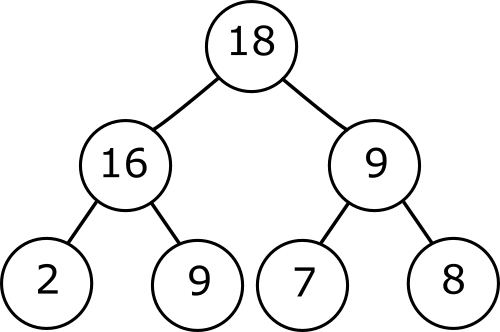
\includegraphics[scale = 0.3]{Images/heap_example.png}
        \caption{Heap Example}
        \label{fig:rsource}
    \end{subfigure}
    ~
    \begin{subfigure}[b]{0.4\textwidth}
        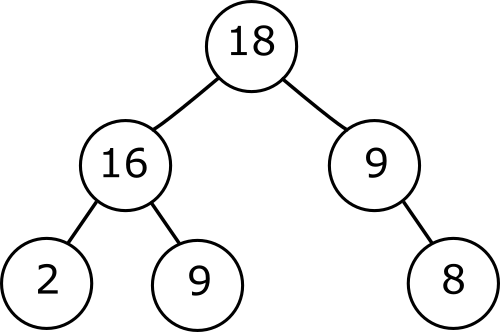
\includegraphics[scale=0.3]{Images/heap_non_example.png}
        \caption{Heap Non-example}
        \label{fig:lsource}
    \end{subfigure}
\end{figure}

The question then becomes how do the different operations work with this structure. The easiest, of course, is \texttt{FindMax} where it only needs return the root of the tree. The other two are a bit more tricky. The general principle when modifying heaps is that we first maintain its shape as a nearly complete binary tree and then modify the values within so that they satisfy the heap property.

Let us first begin with insertion. Given any tree, we know exactly where an additional node should go since every heap of $N$ items has a unique configuration. After a node is added and the value place inside, we compare this added node to its parent to verify whether the heap property is satisfied. If it is, then we are done. If not, we swap the parent and child and ask again whether the newly modified parent (which will contain the inserted value) satisfies the heap property or not. If not, we swap it with its parent again. We continue doing this until the heap property is satisfied or the inserted value reaches the top of the tree. This process is known as ``bubbling up'' or ``max heapifying''. This can occur at most as many times as the height of the tree, so this operation is $\Theta(\log n)$ in the worst case.

\begin{figure}[h]
    \centering
    \begin{subfigure}[b]{0.3\textwidth}
        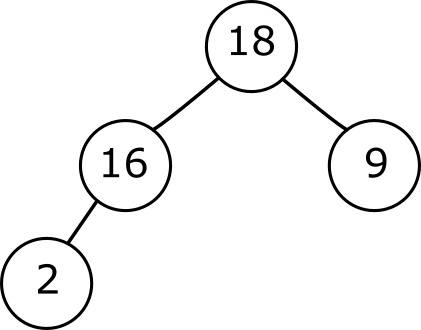
\includegraphics[scale = 0.3]{Images/insertion_step0.png}
        \caption{Starting heap to which we will add 17}
        \label{fig:insert_step0}
    \end{subfigure}
    ~
    \begin{subfigure}[b]{0.3\textwidth}
        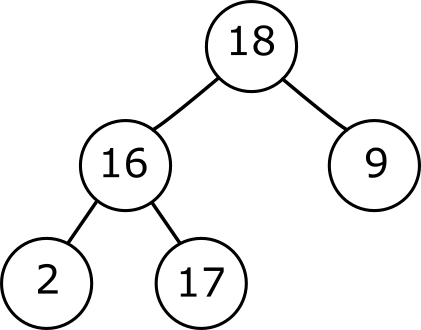
\includegraphics[scale=0.3]{Images/insertion_step1.png}
        \caption{Step1: Add node to maintain heap structure}
        \label{fig:insert_step1}
    \end{subfigure}
    ~
    \begin{subfigure}[b]{0.3\textwidth}
        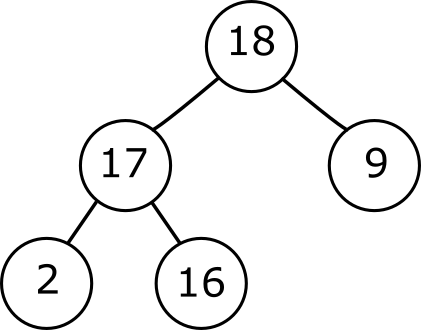
\includegraphics[scale=0.3]{Images/insertion_step2.png}
        \caption{Step 2: Swap 17 and 16 to satisfy the max heap property}
        \label{fig:insert_step2}
    \end{subfigure}
\end{figure}

Extraction of max is a bit more tricky. After we return the maximum value, we remove the very last item of the heap (recall there is only one possible configuartion for any number of nodes, so we know that the last node needs to be removed anyway) and place it as the root. In this case, the heap property is almost certainly not satisfied (although if it is, we are done!). If we need to, we then swap the root with the larger of its children and continue this process of ``bubbling down'' until the heap property is satisfied. Once again this process is $\Theta(\log n)$ in the worst case.

% TODO: Add figure for extract max

\subsection{Array Implementation}
The wonderful thing about heaps is that they can be stored as arrays. This is because, as we've said multiple times, there is unique configuration of a heap for any number of nodes, hence given a list of numbers, we know exactly what heap it would correspond to. The benefit of storing this data as an array is that it becomes very easy to access the children or parent of a node: if a node is at index $i$, its left child will be at index $2i$, its right child is at index $2i + 1$ and the parent is $\lfloor \frac{i}{2} \rfloor$ (Note: this assumes we start indexing from 1 \textit{not} from 0).

\begin{figure}[h]
    \centering
    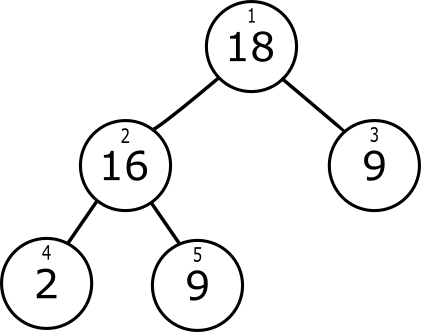
\includegraphics[scale=0.45]{Images/heap_array_tree.png}
    \caption{Heap Example in a tree}
    \label{fig:heap_tree}
\end{figure}
\begin{figure}[h]
    \centering
    
\includegraphics[scale=0.45]{Images/heap_array.png}
    \caption{Same heap in an array}
    \label{fig:heap_array}
\end{figure}

\section{Heapsort}\label{sec:heapsort}
As mentioned heaps are partially sorted. One might wonder how much effort it would take to get it completely sorted, i.e. turn it into a sorted list. We recall that the largest element of the heap is always at the root. So by repeatedly calling \texttt{ExtractMax} on a heap, we should be able to get a sorted list. Remembering that heaps are almost always implemented as arrays, we might get another brilliant insight: do the sorting in place.

For example, we first swap the first and last element in the heap, do the bubbling down and then decrement the heapsize. By decrementing the heapsize, the root which was at the end of the heap is moved out of it. This means that it's already in the position it should be! (assuming we are sorting the list in non-decreasing order).

\begin{figure}[h]
    \centering
    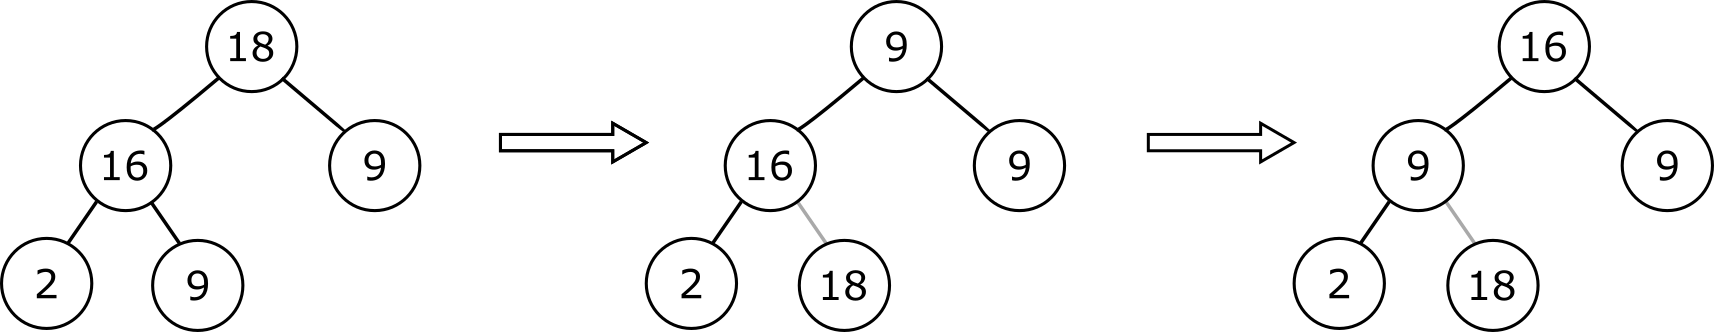
\includegraphics[scale=0.3]{Images/heap_sort_tree.png}
    \caption{Extract max in a tree}
    \label{fig:heap_sort_tree}
\end{figure}

\begin{figure}[h]
    \centering
    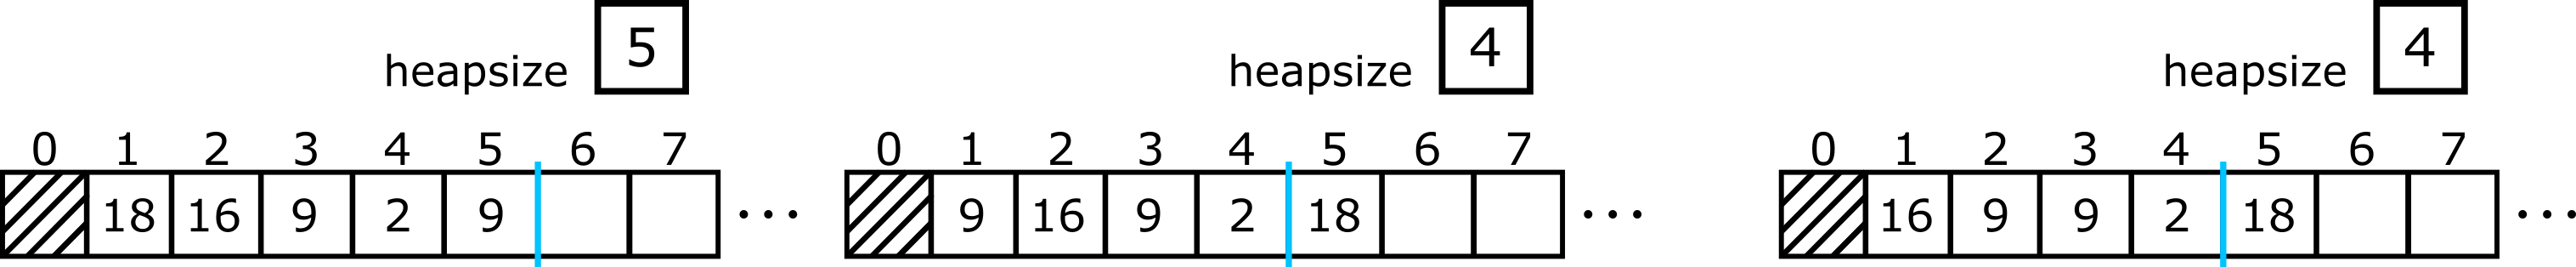
\includegraphics[scale=0.3]{Images/heap_sort_array.png}
    \caption{Extract max in array (note placement of 18). Grey edge indicates removed edge.}
    \label{fig:heap_sort_array}
\end{figure}

As the 18 is past heapsize, we need not worry about it anymore (from the perspective of the heap, it is no longer in it). It is easy to see that as we continue this we will continue placing the largest elements at the end, thereby getting a non-decreasing list at the end.

Let's see what the bubbling-down, also known as MaxHeapify, would look like in code.

\begin{lstlisting}
def maxHeapify(L, i):
    l = left(i) # if 1-based indexing left(i) = 2i
    r = right(i) # if 1-based indexing right(i) = 2i + 1
    if l <= L.heapsize and L[l] > L[i]:
        largest = l # stores index of the largest number
    else:
        largest = i
        
    if r <= L.heapsize and L[r] > L[largest]:
        largest = r
        
    if largest != i:
        exchange L[i] with L[largest]
        maxHeapify(L, largest)
\end{lstlisting}
\vskip.5em

Of course we don't quite have a sorting algorithm yet. We first need to see how to turn an unsorted list into a heap (starting with a heap means if you've already most of the work!).

The most obvious way of turning an unsorted list into a heap would be to start with an empty heap and repeatedly call \texttt{Insert} on the items of the sorted list to add them to the heap. Since \texttt{Insert} preserves the heap property, after all the items have been inserted, we will have a valid heap. Unfortunately, as is so often the case with computer science (and quite frankly life) the most obvious solution is often not very good.

It is easy to see that in the worst case, this algorithm is $O(n \log n)$ since each insert takes at most $\log n$ time and we do $n$ insertions. With a bit more though we can also conclude that this algorithm is also $\Omega(n \log n)$. Recall from above that this requires us to find a family of inputs where the runtime \textit{is} actually $n \log n$. Suppose we apply this algorithm on an increasing list. Then every insertion will take $\log h$ time where $h$ is the height of the tree when the particular insert is called. Note that in any nearly complete binary tree, at least half of the nodes are leaves (induction might be the simplest way of convincing oneself of this fact). These leaves are at a depth of $\log n$ or $\log n - 1$ (if the tree is a complete binary tree then all leaves are at depth $\log n$, otherwise there are some leaves at depth $\log n - 1$). For each of those $\lceil \frac{n}{2} \rceil$ leaves, at least $\log n - 1$ swaps are done. Thus the algorithm is in $\Omega(\lceil \frac{n}{2} \rceil \log(n) - 1)$ which, via asymptotic notation, means that the algorithm is $\Omega(n \log n)$.

Let's see if we can do any better. The problem with the above algorithm is that the most expensive operation is at the leaves which are also the most common node in a heap. Ideally what we would want is an algorithm that is cheap for leaves and maybe a bit more expensive for other nodes. 

One might remember that heaps are recursive in nature. That is, in a heap the left and right child of any node are themselves heaps. Leaves can then be thought of one-node heaps. Inspired by this, and by the previous discussion of \texttt{MaxHeapify}, we might consider the following: put the unsorted array into a nearly complete binary tree and work backwards by calling \texttt{MaxHeapify} on every node. Nodes that are near the bottom of the tree (which are the most frequent ones) have shorter subtrees therefore are cheaper to correct. Indeed this change allows the algorithm to be $O(n)$ rather than $O(n \log n)$.

Let us work this out mathematically. There are $\frac{n}{2}$ leaves (for now we assume $n$ to be a power of 2) hence they are trees of height 0. There are $\frac{n}{4}$ nodes which are rooted at trees of height 1 (these are of course the parents of all the leaves). We continue similarly to conclude that there are $\frac{n}{2^{k}}$ nodes which have trees of height $k - 1$ for $k$ between $1$ and $\log n$. Thus the total time of this algorithm is
\begin{align*}
    \sum_{h = 0}^{\lfloor \log n\rfloor} h \cdot \left\lceil \frac{n}{2^{h + 1}}  \right\rceil = O\left( \frac{n}{2} \sum_{h = 0}^{\lfloor \log n \rfloor} \frac{h}{2^h} \right)
    = O \left( n \right)
\end{align*}
where we use the fact that $\sum_{k = 1}^{\infty} kr^k = \frac{r}{(1 - r)^2}$ provided that $0 < r < 1$ (this is known as Gabriel's staircase series).

\section{Dictionary ADT}
The Dictionary ADT is similar to python's dictionaries. Formally, the data for a dictionary is a set of elements $S$ where each $x \in S$ has a field $x.$key where keys are elements of some totally ordered set (often taken to be the integers). The keys in a dictionary are unique. This means that for every $x, y \in S$ we have that $x.$key $\neq$ $y.$key. The ADT defines 3 operations on this set: \texttt{Insert}, \texttt{Search} and \texttt{Delete}.
\begin{itemize}
    \item \texttt{Insert}($S, x$): Insert $x$ into $S$. If there is some $y$ in $S$ with $y.$key = $x.$key, then replace $y$ with $x$.
    \item \texttt{Search}($S, k$): Return $x$ in $S$ for which $x.$key = $k$. Return null if no such $x$ exists
    \item \texttt{Delete}($S, x$): Delete $x$ from $S$ (note they parameter is $x$, \textit{not} the key)
\end{itemize}

Quite often we think of $x$ as consisting of two parts: the key and everything that is not the key. This remaining part can be called the value of $x$, turning $x$ into the more familiar (\textit{key, value}) pairing.

There are a number of different ways of implementing this ADT, we see some examples below.

\subsection{Direct-Access Table}
Perhaps the simplest way is to create a location in memory for every possible key. For example suppose the only possible keys are numbers 0 -- 99. In this case we can create an array of size 100 and store an inserted value in the appropriate index. In this case, \texttt{Search}, \texttt{Insert} and \texttt{Delete} are all constant time. Of course what we gain in time, we lose in space (if instead the index was given by 32-bit numbers, we would need $2^{32}$ locations in memory!). So we end up reserving an enormous amount of space for ($key, value$) pairs that may never be used.

\begin{figure}
    \centering
    
\includegraphics[scale=0.3]{Images/direct_access_table.png}
    \caption{Direct-access Table}
    \label{fig:dat}
\end{figure}

\subsection{Hash Table}
We can perhaps make things a bit easier by using a hash function. A hash function allows us to map the entire universe of possible keys to a smaller collection and we use this smaller collection to access the table. 

Of course by its very nature, there will be conflicts in this mapping -- the hash function cannot be injective. This means that we need to deal with two different keys being mapped to the same value by the hash function. We discuss this in detail in \autoref{sec:hashing} but a common way of dealing with this is storing the values corresponding to a hashed key as a linked list. In other words each entry in the direct access table for the hashed keys actually points to the head of a linked list. In this worst case, we simply have the items being stored in a linked list which (as we see below) take $\Theta(n)$ time for searching (however the average case can be made $\Theta(1)$ as we will see later, so this is certainly not a bad alternative). Insertion and deleting take $\Theta(1)$ time (assuming we have already searched for the item).

\begin{figure}[h]
    \centering
    
\includegraphics[scale=0.3]{Images/hash_table.png}
    \caption{Hashing keys}
    \label{fig:hash_table}
\end{figure}

\subsection{Array}
Another way we might try to remedy the situation with Direct Access tables is to simply add things to the array when needed, instead of allocating space at the beginning. In this case, when searching we need to iterate over every value in the array in order to determine whether it contains the specified key or not making this $\Theta(n)$. Insertion and deleting however are $\Theta(1)$ (assuming we keep track of the dictionary size, we simply add new items to the corresponding position and after we remove an item we can use the last item to fill the gap. Both of these operations are constant time).

In the above we assume arrays to be unsorted. If we sort the array, then searching becomes $\Theta(\log n)$ (we use binary search) but now insertion and deleting become $\Theta(n)$ since we need to shift items in order to preserve the ordering.

\subsection{Linked List}
With an unsorted linked list the situation is much the same as before, searching is $\Theta(n)$ while insertion and deleting are quite cheap, being constant time (as always, we assume the insertion and deletion happen \textit{after} a search is performed, so we don't account for the time spent on searching). The situation remains exactly the same if we sort the linked list instead since we cannot access the central element of the list in order to perform binary search.

\subsection{Binary Search Tree}
The above seems to very strongly suggest using a binary search tree since we point directly to the central element! Unfortunately in the worst case a binary search tree could be completely one-sided an simply be a linked list. If only there were some way of ensuring that a binary tree were balanced...

\subsection{Balanced Search Trees}
This is of course what inspires the category of what are called balanced search trees that try to minimise the height of a tree as much as possible. There are many different kinds such as red-black trees, AVL trees, B trees, etc. We will look at AVL trees.

\section{Binary (Search) Trees}
We take a brief refresher with binary trees before delving into how to balance them.

A binary tree is simply a tree where each node has at most 2 children. As usual, if a node has no child it is called a leaf. The height of a tree is the size of the longest path between the root and its leaves (where the size of the path is given by the number of edges traversed, in particular then a single node tree is of height 0). The depth of a node is the size of the path from the root to that node. We can then equivalently define the height of the tree as the maximum depth of any node in the tree.

A binary tree is called a binary search tree if every node satisfies the binary search tree property: everything on the left subtree of a node is smaller than or equal to the node and everything on the right is greater than or equal to the node.


\begin{figure}[h]
    \centering
    
\includegraphics[scale=0.3]{Images/non_bst.png}
    \caption{Example of non-BST}
    \label{fig:non_bst}
\end{figure}
\begin{figure}[h]
    \centering
    
\includegraphics[scale=0.3]{Images/bst_example.png}
    \caption{Example of BST}
    \label{fig:bst_example}
\end{figure}

\subsection{Insert}
Now we consider how we might implement the Dictionary ADT using a binary search tree. First we recall that the keys of a dictionary are unique, so we know that everything on the left subtree is going to strictly smaller than the root which in turn is going to strictly smaller than everything on the right subtree. The insertion algorithm for a BST might look something like so\\
\begin{lstlisting}[language=Python]
INSERT(S, x):
    # Helper may need to modify the root itself: have it return value.
    S.root <- TREE-INSERT(S.root, X)
    
TREE-INSERT(root, x):
    if root is NIL: # x.key not already in S
        # Found insertion point: create new node with empty children
        root <- TreeNode(x)
    else if x.key < root.item.key:
        root.left <- TREE-INSERT(root.left, x)
    else if x.key > root.item.key:
        root.right <- TREE-INSERT(root.right, x)
    else: # x.key == root.item.key
        root.item <- x # replace root with x
    return root
\end{lstlisting}
\begin{remark}
    Note that $S$ doesn't technically store the whole tree. It only stores (a pointer to) the root and we can recursively go through the tree using \ttt{.left} and \ttt{.right}.
\end{remark}

It is then clear that the runtime for \ttt{Insert} depends on the the height of the tree. Also note that the same set of numbers could give us completely different trees, depending on the order in which they are inserted (see \autoref{fig:rough_balanced_bst}). We will see that this is a primary concern with binary trees.

\begin{figure}[h]
    \centering
    
\includegraphics[scale=0.15]{Images/insertorder1.png}
    
\includegraphics[scale=0.15]{Images/insertorder2.png}
    \caption{Dependence of BST on insertion order}
    \label{fig:rough_balanced_bst}
\end{figure}

\subsection{Search}
An algorithm for \ttt{Search} can be described like so
\begin{lstlisting}
SEARCH(S, k):
    return TREE-SEARCH(S.root, k)
    
TREE-SEARCH(root, k):
    # Compare root.key with k to determine if k is to the left or right
    # return when root.key == k
    if root is NIL: # k not in S
        pass
    else if k < root.key:
        root <- TREE-SEARCH(root.left, k)
    else if k > root.key:
        root <- TREE-SEARCH(root.right, k)
    else: # we have found the key
        # root.key == k
        pass
    return root
\end{lstlisting}

Once again the runtime is dependent on the height of the tree, which in the worst case is simply the number of items.


For illustrative purposes, we can analyse the expected number of calls to search among the two trees above in \autoref{fig:rough_balanced_bst}, assuming that $k$ is chosen uniformly from $\{0, \dots, 10\} \backslash \{9\}$. We note that there are $d + 1$ calls to \ttt{TREE-SEARCH} to find a node a depth $d$. The probability of choosing any node is simply $\frac{1}{10}$. Thus for the first binary tree, the expected number of calls is
\begin{align*}
    E(T_1) = &\sum_{n} P(k = n)(\text{number of \ttt{TREE-SEARCH} calls to find node }n)\\
    &=\frac{1}{10}(1 \cdot 1 + 2 \cdot 2 + 3 \cdot 3 + 4 \cdot 3 + 5 \cdot 1) = 3.1
\end{align*}

For the second binary tree, as every node is at a different depth, we simply have
\begin{align*}
    E(T_2) &= \sum_{k = 1}^{10} \frac{1}{10} \cdot k\\
    &= \frac{1}{10} \cdot \frac{10 \cdot 11}{2}\\
    &= 5.5
\end{align*}
As one would expect, the taller tree on the right will require more function calls on average.

\subsection{Delete}
There are three distinct cases to consider when deleting from a BST. The easiest case is when we are asked to delete a leaf-- we simply delete. If the node has only one child, then the task is also quite straightforward, we promote the sole child to the place of the deleted node. The difficult case is when deleting a node that has two children. In this case, we can replace the node we want to delete with the predecessor (the rightmost node on the left subtree) or the successor (the leftmost node on the right subtree).
\begin{remark}
    In this course, we \textbf{always} replace the deleted node with the successor.
\end{remark}

We have the following algorithm for this
\begin{lstlisting}
TREE-DELETE(root, x):
    if root is NIL: # x.key not in S, should not happen
        pass
    else if x.key < root.item.key:
        root.left = TREE-DELETE(root.left, x)
    else if x.key > root.item.key:
        root.right = TREE-DELETE(root.right, x)
    else: # x.key == root.item.key so we remove root.item
        if root.left is NIL:
            root = root.right # NIL if both children missing
        else if root.right is NIL:
            root = root.left
        else:
            # Means root has two children
            # Want to remove min item in right subtree
            # Assumption: DELETE-MIN returns two values:
            # - element removed from right subtree
            # - root of resulting subtree
            root.item, root.right = DELETE-MIN(root.right)
            
DELETE-MIN(root):
    # Remove element with smallest key in root's subtree
    # return element that was removed and root of resulting subtree
    if root.left is NIL:
        # Root stores item with smallest key; replace with right child.
        return root.item, root.right
    else:
        # Left subtree not empty; root not the smallest
        item, root.left = DELETE-MIN(root.left)
        return item, root
\end{lstlisting}

As usual the runtime of this is dependent on the height of the tree which we can minimise by balancing the tree.

\subsection{Duplicate Keys}
We take a brief segue to discussing the problem of how one may implement a Dictionary ADT that allows for duplicate keys to occur using a BST. There are various strategies for how one may deal with duplicate values. In this case we will analyse the different strategies by considering what happens in the case when we try to insert $n$ identical items. 

The simplest strategy we could have for handling duplicate keys is to always put duplicates in the right subtree. We can easily modify the code for \ttt{TREE-INSERT} in order to achieve this.

\begin{lstlisting}
INSERT(S, x):
    # Helper may need to modify the root itself: have it return value.
    S.root <- TREE-INSERT(S.root, X)
    
TREE-INSERT(root, x):
    if root is NIL: # x.key not already in S
        # Found insertion point: create new node with empty children
        root <- TreeNode(x)
    else if x.key < root.item.key:
        root.left <- TREE-INSERT(root.left, x)
    else:
        root.right <- TREE-INSERT(root.right, x)
    return root
\end{lstlisting}

Now we consider our test case of inserting $n$ duplicates into an empty tree and ask how much time this takes. Assume that one call to \ttt{TREE-INSERT} takes time $c$. At depth $k$, we need to make $k + 1$ calls to \ttt{TREE-INSERT}. Therefore the time taken to insert $n$ duplicate items is
\begin{align*}
    \sum_{k = 1}^{n} k = \frac{n(n + 1)}{2}
\end{align*}
Thus the operation is $\Theta(n^2)$ for this case.

An alternative we might consider is to alternate going left and right. In particular, we add a boolean flag to each node, which dictates whether duplicates should go to the left or the right. Then each time a duplicate is inserted, the flag is inverted so that the next duplicate will be inserted in the opposite direction.

% TODO: Add diagram for boolean flag method

Let us try our test case again. We see that the height of the final tree (after all $n$ items are inserted) is $\log n$. In fact if the tree has $m$ items at a stage it will take $\Theta(\log m)$ time to insert another item. Therefore the total time taken is
\begin{align*}
    \sum_{m = 1}^{n} c \log m = c \sum_{m = 1}^{n} \log m < c \sum_{m = 1}^{n} \log n = c n \log n
\end{align*}
Hence the insertion is now $O(n \log n)$, a considerable improvement! Let us show that we are in fact in $\Theta(n \log n)$.
\begin{align*}
    \sum_{m = 1}^{n} c \log m > \sum_{m = \frac{n}{2}}^{n}c \log m > c \sum_{m = \frac{n}{2}}^{n} \log \left(\frac{n}{2}\right) = c \frac{n}{2} \log \left( \frac{n}{2} \right) = \frac{c}{2}(n \log n - 1)
\end{align*}
\begin{remark}
    Note the `trick' above of only considering half the sum. This is a useful technique for finding lower bounds.
\end{remark}
Thus with this approach we are in $\Omega(n \log n)$ as well implying that we are indeed taking $\Theta(n \log n)$ time.

\section{AVL Trees}
Everything we have done so far suggests that we want our trees balanced so that searching (and therefore inserting and deleting) can be optimised. However keeping a tree balanced also uses up resources as we also need to maintain the BST property (what this means before we move nodes and subtrees around we need to find appropriate places for them). Much like with heaps, the solution is a compromise: we allow the trees to be slightly imbalanced so that searching can be fairly fast (the tree is mostly balanced) but we don't need too much maintenance every time we insert or delete (the tree is \textit{mostly} balanced). This is what AVL trees do.\\

We need first define how we are going to be decide whether a tree is (sufficiently) balanced. We do this using the balance factor. The balance factor ($BF$) of a node $m$ is
$$BF(m) = h_R - h_L$$
where $h_R$ is the height of the right subtree and $h_L$ is the height of the left subtree.
\begin{remark}
We say that the height of the empty tree is $-1$ so that we may distinguish it from a one node tree.
\end{remark}
If $BF(m) = 0$ then the tree (rooted at $m$) is balanced. If $BF(m) = 1$ then the tree is right heavy but still AVL balanced. Similarly if $BF(m) = -1$ then the tree is left heavy but also remains AVL balanced. However if the balance factor is any other value, it is no longer AVL balanced. A binary tree is an AVL tree if and only if the balance factor of all of the nodes is between $-1$ and $1$ (inclusive). This final property is known as the AVL invariant.

\begin{figure}[h]
    \centering
    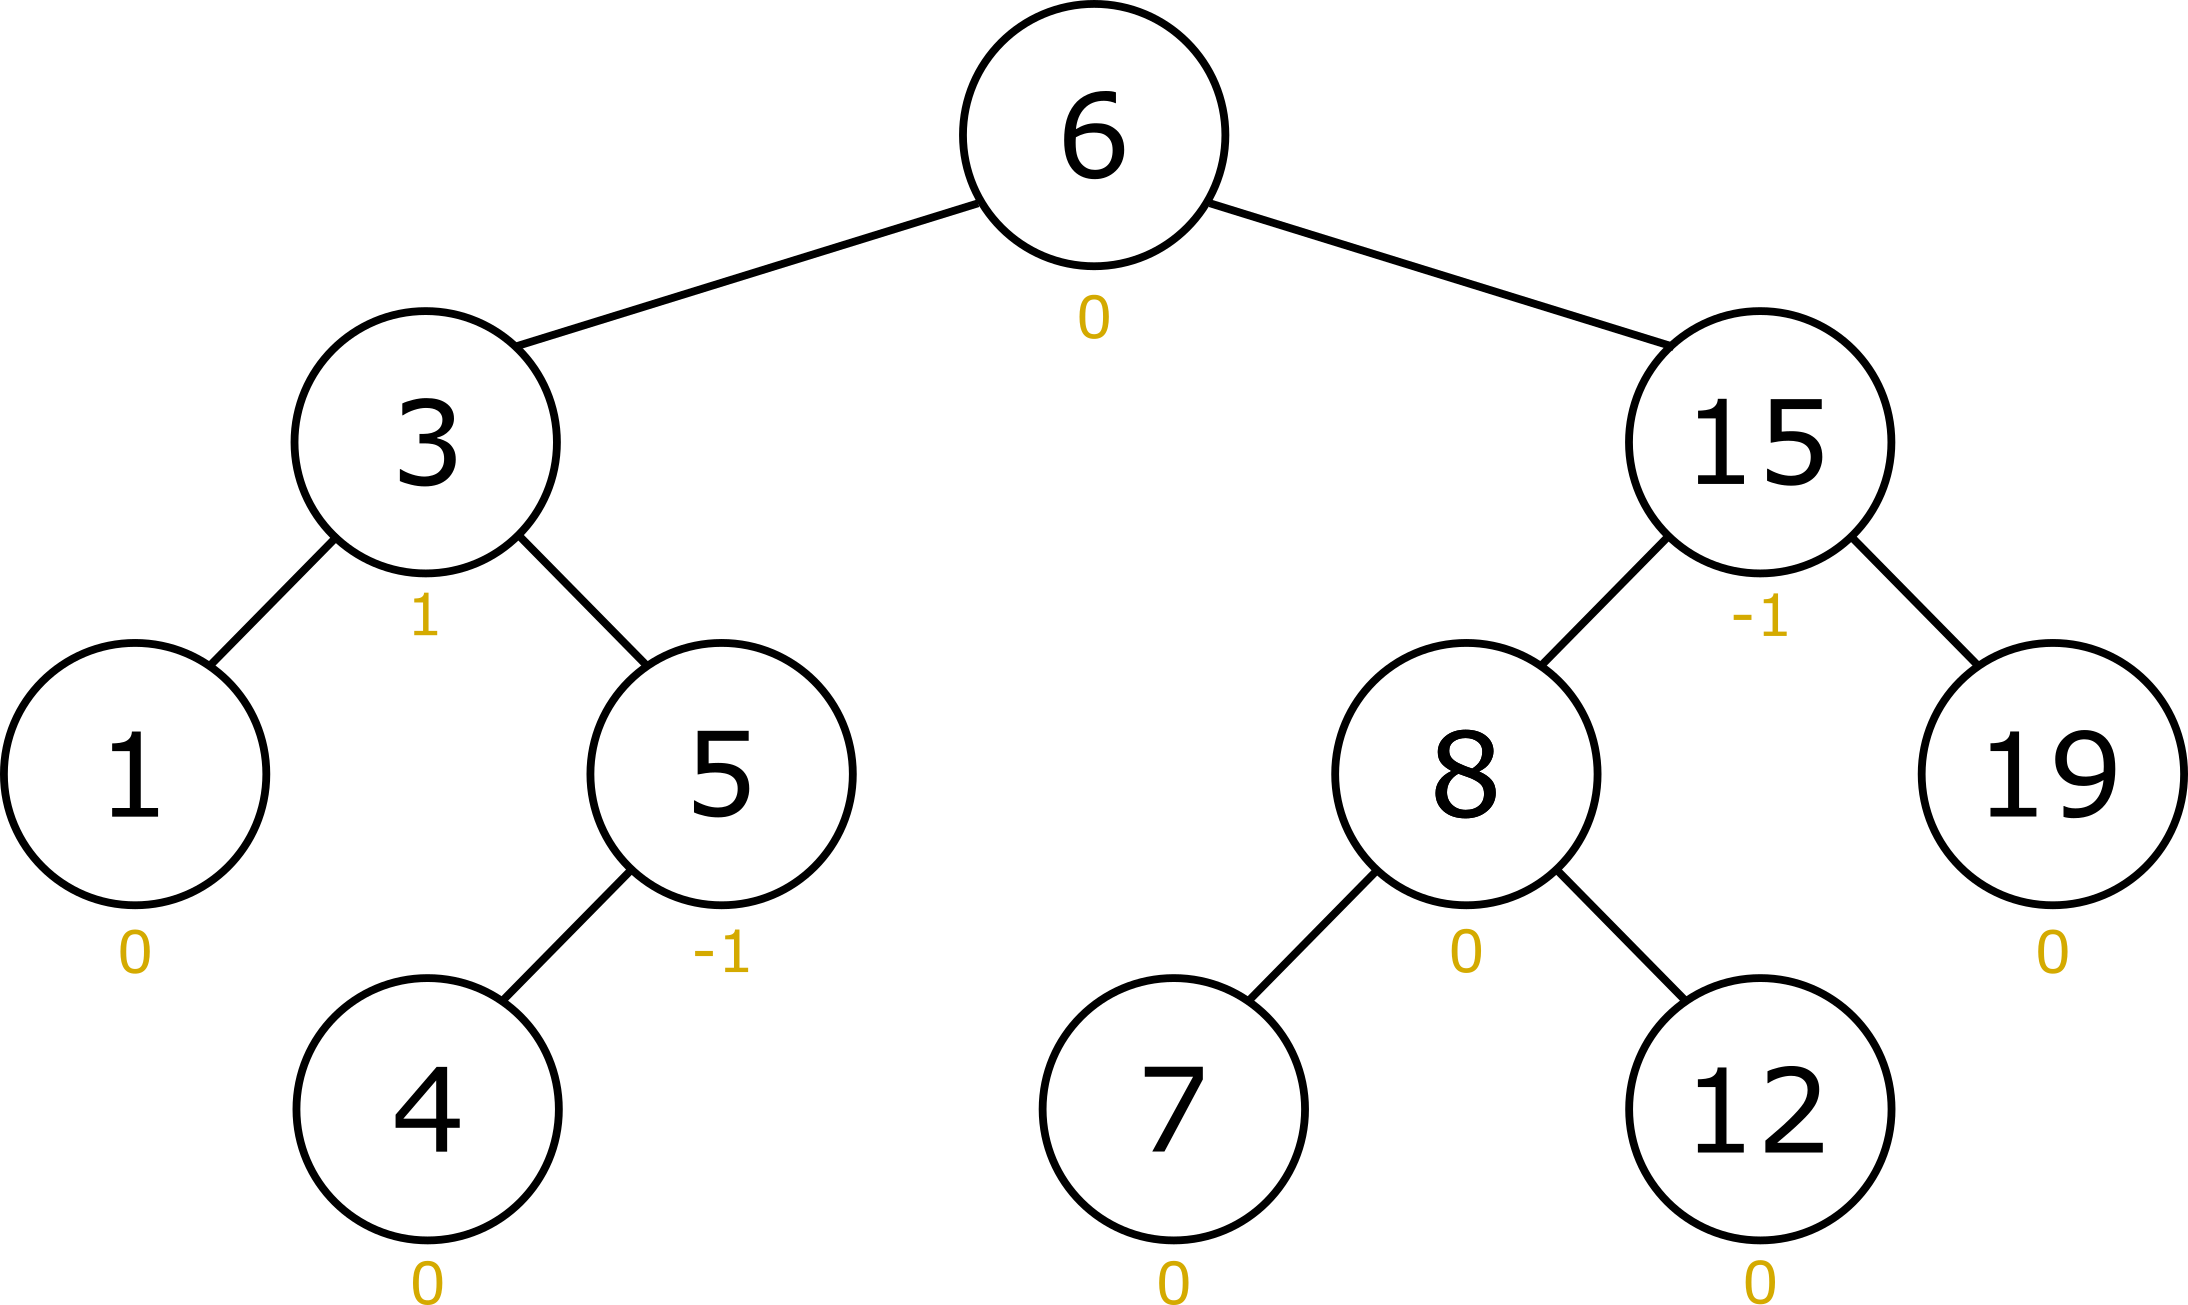
\includegraphics[scale=0.25]{Images/avl_example.png}
    \caption{Example of an AVL Tree (balance factors in yellow)}
    \label{fig:avl_example}
\end{figure}

Searching in an AVL tree is easy since it's still a binary search tree. Thus the interesting operations are \ttt{Insert} and \ttt{Delete} as these may cause the tree to no longer be AVL anymore. Thus we need ways of correcting trees that have been knocked out of balance.

\subsection{Insert}
We first consider the case with insertion. It often helps to name things, so let $T$ denote our AVL tree and let $x$ be the item we are inserting. Note that when we insert $x$, the only balance factors that could possibly change are the ancestors of the newly inserted node (see \autoref{fig:avl_insertion}). This is because by definition the balance factor at a node is $h_R - h_L$. The height of the right or left subtree at any node can only change if the node is an ancestor of $x$ (that's exactly what it means to be an ancestor!). Hence the balance factors for non-ancestral nodes remain the same.

\begin{figure}[h]
    \centering
    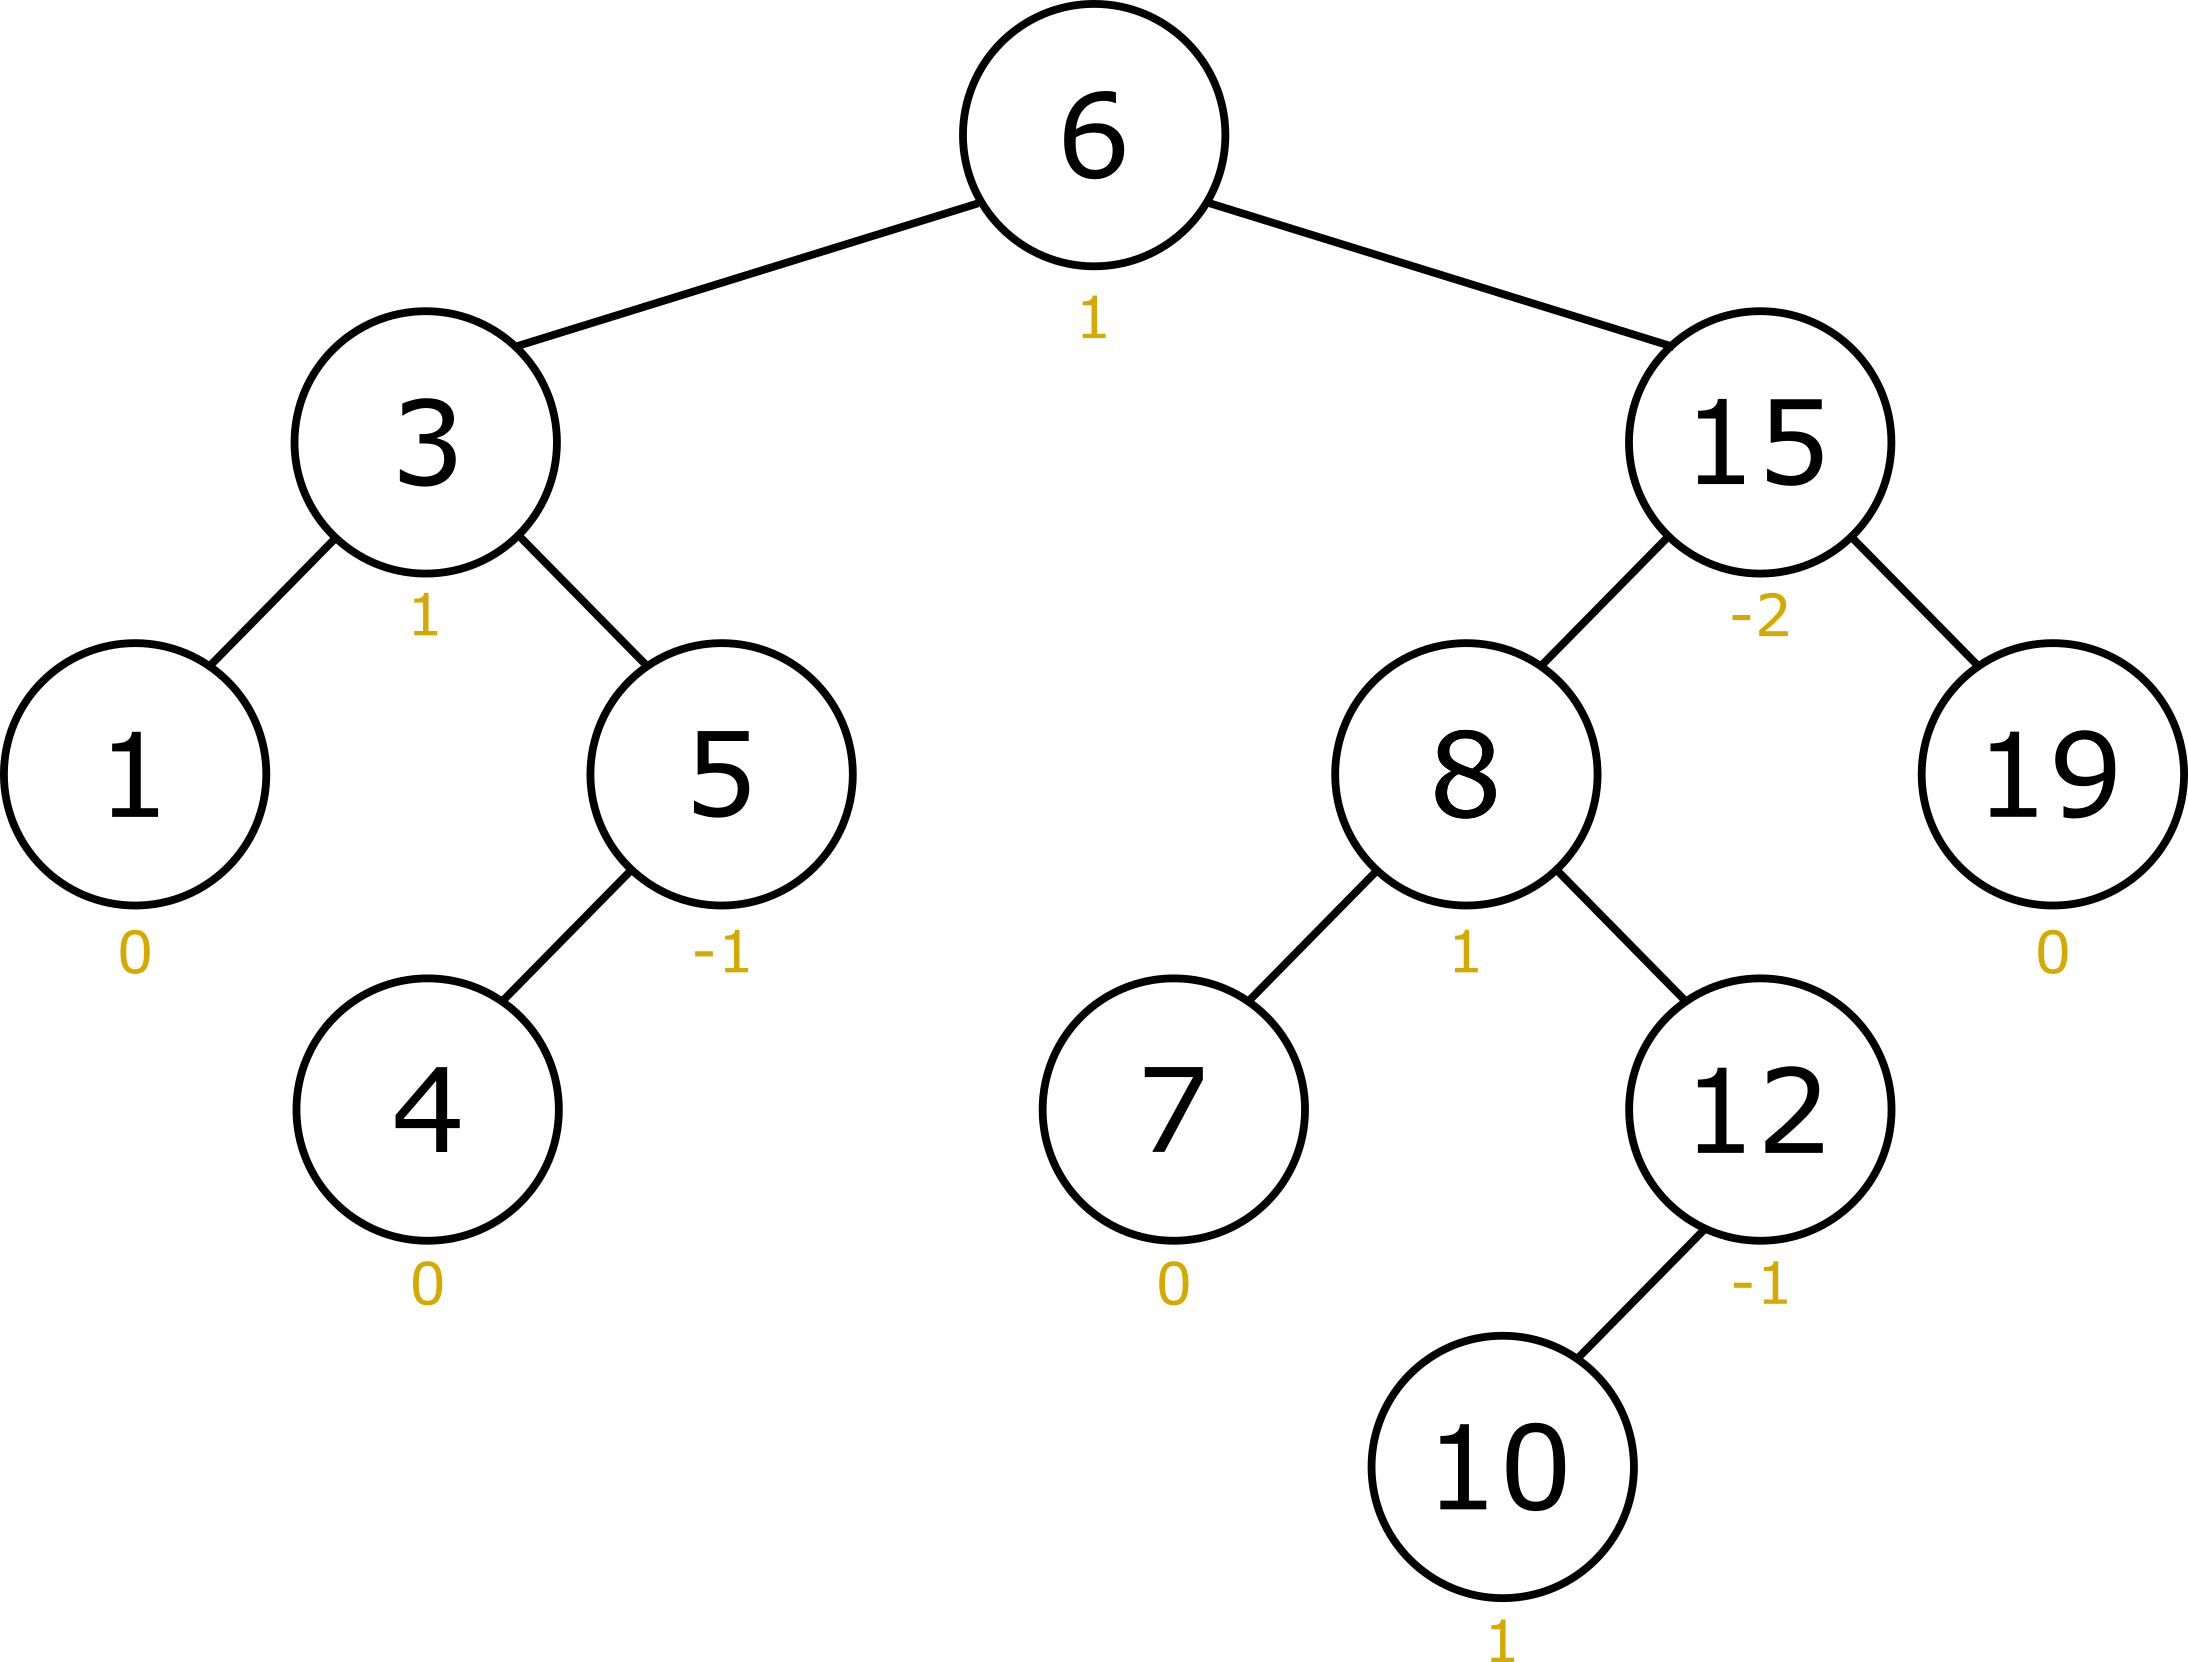
\includegraphics[scale=0.25]{Images/avl_insertion.png}
    \caption{Inserting into an AVL tree (compare with \autoref{fig:avl_example} to note the balance factors that changed)}
    \label{fig:avl_insertion}
\end{figure}

The only way inserting $x$ can knock $T$ out of balance is if we insert into the right subtree of a right heavy tree or the left subtree of a left heavy tree. The symmetry of the situations means we only need consider one of those cases; we choose the former.

% TODO: Add names and depths to figure
\begin{figure}[h]
    \centering
    
\includegraphics[scale=0.7]{Images/avl_insert_out_of_balance.png}
    \caption{Inserting makes AVL tree out of balance}
    \label{fig:oob_avl_tree}
\end{figure}

Even within this there are 2 (unfortunately asymmetric) cases to consider. But first we need more names: let $m$ be the `lowest ancestor' (i.e. with the ancestor with the greatest depth) of $x$ that is no longer AVL-balanced after the insertion of $x$. As we will see it suffices to fix the subtree rooted at $m$, so we will assume $m$ to be the root. Let $T_1$ be the left subtree of $m$, let $m_R$ be $m$'s right child with left and right subtrees $T_2$ and $T_3$ respectively. Suppose $T_1$ is of height $h$. We assumed $T$ to be right heavy implying that $m$'s right subtree (i.e. the tree rooted at $m_R$) is of height $h + 1$. 

Our first claim is the following.
\begin{lemma}
    $T_2$ and $T_3$ are both of the same height and in particular are of height $h$.
\end{lemma}
\begin{proof}
    We know that before the insertion of $x$, the balance factor of $m$ was 1 (recall we are assuming that we insert into the right subtree of a right heavy tree). Since the height of $m$'s left subtree was $h$, the height of its right subtree must be $h + 1$. This means that at least one of $m_R$'s subtrees, i.e. one of $T_2$ and $T_3$, is of height $h$. Without loss of generality we can assume it to be $T_2$ (this is one of those symmetric cases). Suppose $T_3$ is not of height $h$, then it must be of height $h - 1$ (by the AVL property we know the only possible heights for $T_3$ are $h, h + 1$ and $h - 1$. We assume it is not $h$ and if it was of height $h + 1$ then the tree rooted at $m$ would not have been AVL at the beginning). Since the insertion of $x$, knocks $m$ out of balance, we know it must be inserted in to $T_2$ (if it was inserted into $T_3$, $BF(m_R)$ would remain unchanged). This causes the height of $T_2$ to increase to $h + 1$ (if this height did not change then $BF(m_R)$ would again remain unchanged). But then $m_R$ is out of balance since its balance factor is now $(h - 1) - (h + 1) = -2$. However we assumed that $m$ was the lowest ancestor to be knocked out of balance, leading to a contradiction.
\end{proof}

Now that we have that sorted (ha!), we need to consider how to correct the tree after inserting $x$. As mentioned we split this into two cases, inserting into $T_2$ and inserting into $T_3$. The simpler case is inserting into $T_3$ so let us start with that. In this case, we can fix the tree with what's called a \textit{single (left) rotation} (if we were inserting into the left subtree of $m$'s left child we would do a single right rotation instead). This is most easily illustrated via diagrams. 

\begin{figure}[h]
    \centering
    
\includegraphics[scale=0.6]{Images/avl_single_rotations.png}
    \caption{AVL (single) rotations}
    \label{fig:avl-sing-rotation}
\end{figure}

There are some important properties that the single rotation has:
\begin{minitemize}
    \item The tree rooted at $m$ is now balanced
    \item The BST property is maintined
    \item The rotation takes constant time (in fact only 3 pointers are changed)
    \item The height of the tree (rooted at $m$) is the same after the insertion + rotation as it was before the insertion
\end{minitemize}
The last one is a particularly important property. It means that after we have performed a single rotation to fix the balance, the rest of tree (above $m$) is also balanced now. Thus no more work needs to be done!

There is, however, work needing to be done for finishing the remainder of the algorithm. The only case that remains to be considered is if we insert $x$ into $T_2$. In this case (as you can check) a single rotation is not enough to fix the problem. However, if we stare long and hard, we might realise that performing a single right rotation on $m_R$ gets us to the previous case (where the insertion was on the right subtree of the right child of $m$). Therefore, to fix this case, we first rotate right on $m_R$ (to get a right-right heavy tree) and then rotate left on $m$ to get a balanced tree. This is called a \textit{double rotation}, with this specific process being called a double right left rotation (if we had inserted into $m_L$'s right subtree we would do a double left right rotation instead). Note that double rotations share the same properties that single rotations do (admitted a few more pointers need to changed but the operation remains constant time).

% TODO: Add diagram of double right left rotation

Let us then see what this algorithm looks like.

\begin{lstlisting}[language=, numberstyle=\color{white}]
INSERT(T, x):
Insert x into T as you would in a BST

Set BF of x to 0 and retrace path from x to root. For every node m:
i) if x was in m's right subtree, increment BF(m) by 1, if x was in m's left subtree, decrement BF(m) by 1.
ii) If BF(m) == 1 or BF(m) == -1, continue
iii) If BF(m) == 0, stop (an unbalanced tree is now balanced, no change needs to be made to ancestors)
iv) If BF(m) == 2 and BF(m_R) == 1, do a left rotation on m and stop
v) If BF(m) == 2 and BF(m_R) == -1, do a double right left rotation on m and stop
vi) If BF(m) == -2 and BF(m_L) == 1, do a double left right rotation on m and stop
vii) If BF(m) == -2 and BF(m_L) == -1, do a single right rotation on m and stop
viii) If m is the root, stop
\end{lstlisting}

\subsection{Delete}
The first thing to note with delete is that all cases boil down to deleting a leaf. Recall that there are 3 cases to consider when deleting from a BST: deleting a node with 0 children (i.e. a leaf), deleting a node with 1 child and deleting a node with 2 children. The first case remains the same. For the second case, with AVL trees, this necessitates that the sole child of the node is a leaf (otherwise we would be out of AVL balance). Thus we way swap this node with its child and then delete the leaf. For the last case, we swap the node with its successor, which is either a leaf or has one (right) child, getting us to previous cases in either case. Thus we only consider the case of deleting a leaf. For the remainder of this (sub)section any deletion can be assume to be of a leaf.

Once again there are two symmetric cases that cause an imbalance: deleting from the left subtree of a right heavy tree or deleting from the right subtree of a left heavy tree. As before we will only consider one case, the former one. The setup is the same as before: $m$ is the lowest ancestor of $x$ that is now out of balance. We denote its right subtree $T_3$ and it's left child $m_L$. The left and right subtrees at $m_L$ are called $T_1$ and $T_2$ respectively. We will again assume $T_3$ to be of height $h$ after the deletion of $x$ (so the height of $m$'s right subtree would have been $h + 1$ before deletion). Since $m$ is now too left heavy, we know its balance factor is $-2$. This means that the height of $m$'s left subtree is $h + 2$ hence at least one of $T_1$ and $T_2$ is of height $h + 1$. Let us first consider the case with $T_1$ being of height $h + 1$ (and $T_2$ can be of height $h$ or height $h + 1$). See \autoref{fig:avl-delete-case1} for the diagram. In this case we see that a single right rotation on $m$ rebalances the tree. One important thing to note, however, is that if $T_2$ is of height $h$, the height of tree after the rotation is \textit{is not the same as it was before deletion} but has been decremented by 1. We will return to this point later. For now we deal with the case where $T_1$ is of height $h$.

\begin{figure}[h]
    \centering
    
\includegraphics[scale=0.5]{Images/avl_delete_case1.png}
    \caption{AVL Deletion case 1}
    \label{fig:avl-delete-case1}
\end{figure}

In the other case (with $T_2$ being of height $h + 1$ and $T_1$ of height $h$), as one might guess, we will need a double rotation (specifically a left right rotation). This being a bit more delicate operation, we should provide some more details. So first, names: let $m_{LR}$ be the right child of $m_L$ with left and right subtrees $T_{21}$ and $T_{22}$ respectively. Since we assume $T_2$ to be of height $h + 1$, we know that at least one of $T_{21}$ and $T_{22}$ is of height $h$. See \autoref{fig:avl-delete-case2} for the diagram. After the double rotation (a left rotation on $m_L$ followed by a right rotation on $m$), we see that $m_L$'s right child is now $T_{21}$ (the left child of course remains the same: $T_{1}$).
$m_{LR}$ is now at the root with $m$ as its right child ($m_L$ remains as the left child to the root). We see that $m$'s left child is now $T_{22}$ and the right child is now $T_3$. In particular this means that the height of $m_{LR}$'s left and right subtree (which remember is the root now) is $h + 1$ therefore the height of the tree rooted at $m_{LR}$ is $h + 2$. Since the tree was of height $h + 3$ before the deletion, in this scenario we are guaranteed to decrease the height of the tree.

\begin{figure}[h]
    \centering
    
\includegraphics[scale=0.5]{Images/avl_delete_case2.png}
    \caption{AVL Deletion case 2}
    \label{fig:avl-delete-case2}
\end{figure}

The fact that trees may change height means that the balance factor of their parents may change and may cause these nodes higher up to be out of AVL balance. Thus after these rotations, we need to check that $m$'s parent is still in AVL balance and fix it via rotations again if not. How far do we need to continue this? If the height of the tree rooted at $m$ hasn't changed then we don't need to do anything of course. So suppose the height of $m$ has decreased. If $m$ was a left child, the balance factor of its parent increases by 1 and if it was a right child, the balance factor decreases by 1. If the parent $p$ was originally balanced then its going to be left or right heavy now but the height of tree rooted at $p$ has not changed ($m$'s sibling remains of the same height) therefore we don't need to do anything further up. If instead $BF(p)$ was originally $-1$ or 1 is now 0 then we've definitely made the tree shorter so we need check that the balance factor of its parent is fine. If the balance factor went from $-1/1$ to $-2/2$ then we do some rotations. If the tree is restored to its original height then no more works needs to be done. As usual though if the height has been shortened then we must check its parent and repeat the whole process. We summarise all this into the algorithm below.

In the worst case, we could end up making corrections all the way up to the root, totalling $O(\log n)$ rotations. Luckily with the rotations being constant time, this means this deletion algorithm is still $O(\log n)$. We end with the deletion algorithm written in full.

\begin{lstlisting}[language=, numberstyle=\color{white}]
DELETE(T, x):
Find node (leaf) x to delete

Trace the path back to the root. For every node m:
If BF(m) was previously 0:
    Update BF and exit. No further work needs to be done since the height of the tree rooted at m has not changed.
If BF(m) was previously -1 or 1 and is now 0:
    The tree rooted at m is now shorter. This may affect m's ancestors so we continue moving up the tree.
If BF(m) was previously -1 or 1 and is now -2 or 2:
    Perform the appropriate rotation. If the height of the tree rooted at m is the same, we can quit. If it has changed we continue moving up the tree
\end{lstlisting}

\subsection{Key Ideas}
There is often a competition that occurs between operations: optimising one operation to its maximal point often comes at the cost of making other operations more expensive (ideally we would like to maintain a perfect BST for above but this makes insertion and deletion too expensive). Hence we strike a compromise between these to make all operations relatively fast. This is a key (and as you can see recurring) idea when designing algorithms.

Another important note is that by storing extra information on existing data structures, we can improve those data structures (after all AVL trees are simply BSTs with the additional BF data!). This is known as augmenting data structures (see the following section). This lightly highlights another tension in computer science: we can often save on runtime by sacrificing space (i.e. memory) and vice versa. Our goal is to find an optimal balance between the two.

\section{Augmented Data Structures}\label{sec:aug-data-struc}
As mentioned, augmenting data structures is the idea of storing additional information in our data structures to allow us to do additional operations reasonably fast, while still maintaining the efficiency of our previous operations. This latter part is often the difficult bit. We will study this via an example.

Given an ordered set, we say that the rank of an element is its position in the set (for example the rank of the first element would be 1). With this definition, we would like to augment an AVL tree to have the following operations:
\begin{minitemize}
\item \ttt{RANK}($k$): Return the rank of key $k$
\item \ttt{SELECT}($r$): Return the key with rank $r$
\end{minitemize}
As these still remain AVL trees, we still want to maintain the operations of \ttt{INSERT}, \ttt{SEARCH} and \ttt{DELETE}. 

Without any modification to AVL trees, the new operations are $\Theta(n)$ (we effectively have to do an in order traversal through the tree to determine what position a particular node is in). A better suggestion appears to be to have each node store its rank. Now the new operations become $\Theta(\log n)$ (\ttt{RANK} simply requires searching for $k$ while for \ttt{SELECT} we run binary search on the rank itself) which seems rather promising but then we realise that the operations of \ttt{INSERT} and \ttt{DELETE} become $\Theta(n)$ as any changes to the tree may require us to update the ranks of all the nodes. 

As before we need some kind of compromise. Something that allows us to find the rank of a node (relatively) easily and is also (relatively) easy to maintain. With a bit of stumbling around or by asking someone smarter than us, we may come across the following idea: have each node store its size, which is defined to be the number of nodes in the subtree rooted at that node (so the size of a leaf would be 1, the size of a complete binary tree of height 1 would be 3, etc). For one this allows us to use binary search to find a node of some particular rank. For example suppose we are looking for rank 4 and \ttt{root.size} is 7. If \ttt{root.left.size} is also 4 then we immediately know that the node we seek is in the left subtree and we need not bother at all with the right subtree. At this point we can repeat the process by looking at the left and right children again. If we were looking for rank 6 instead, then we would know that the desired node is in the right subtree. Additionally we can work out that 5 elements appear before the right child $R$ (4 in left subtree + 1 for the root itself). Thus we seek for the 1st element, or the node of rank 1, in the right subtree. The recursive structure of this algorithm now becomes clear. As a remark, we mention that \ttt{node.left.size + 1} is a very common calculation we will be doing and has a very natural interpretation: it is the rank of the root of the subtree rooted at that node. We call this quantity the local rank. As a further remark to the remark, recall that trees themselves have a recursive structure. Although this may seem obvious, this is a useful thing to remember when constructing algorithms for trees. In particular we might be able to make statements about the whole tree (i.e. a global statement) by working things out on/from the left and right subtrees (local statements).

The algorithm for \ttt{SELECT} may, then, look something like this
\begin{lstlisting}
SELECT(T,r):
    if T.left != NIL:
        local_rank = T.left.size + 1
    else:
        local_rank = 1 # if left tree is empty then the root is first element hence has rank 1
        
    if local_rank == r:
        return T.root
    if k < local_rank:
        return SELECT(T.left, r)
    else:
        return SELECT(T.right, r - local_rank)
\end{lstlisting}

Now we look at \ttt{RANK}. This means given a key $k$, we need to find how many elements less than $k$ are in the tree. Consider how we might do so while traversing the tree in order to find $k$. If $k$ is in node $m$'s right subtree then we know that at least \ttt{local\_rank}($m$) elements come before it. If $k$ is in the left subtree instead, we can make no further inferences (well, the the size of the left tree gives us an upper bound for the rank of $k$. So we are still cutting down the space of possibilities. However there is little we can do to use this information directly). This suggests keeping a running total as travel down the tree.

\begin{lstlisting}
RANK(T, k):
    return  TREE-RANK(T, k, 0)
    
TREE-RANK(T, k, current_rank):
    if root is NIL: # k not in T
        pass
    # determine local_rank
    if root.left is NIL:
        local_rank = 1
    else:
        local_rank = root.left.size + 1
    
    if k < root.item.key:
        # moving left so can't deduce anything
        return TREE-RANK(T, k, current_rank)
    if k > root.item.key:
        # add the number of items we have skipped
        return TREE-RANK(T, k, current_rank + local_rank)
    if k == root.item.key:
        return current_rank + local_rank
\end{lstlisting}

The time for this implementation of \ttt{SELECT} and \ttt{RANK} are $\Theta(\log n)$ (we are effectively doing some version of binary search in both cases while keeping track of some additional information. Once again a common technique to use with trees to cut the space of possibilities in half each time). However, importantly, the old operation of \ttt{INSERT}, \ttt{SEARCH} and \ttt{DELETE} are still $\Theta(\log n)$! This is because when inserting or deleting we only need change the size attribute of the node being inserted/deleted and its ancestors.

Unfortunately, we can't pat our backs quite yet. Recall theses are AVL trees and there is another operation that can be performed on such trees (and indeed often is). I speak, of course, of rotations. We need ensure that rotations are still constant time when maintaining the size attribute. However this is easily verified since rotations only change the sizes of two nodes (the root and one of its children depending on the direction of the rotation) and new sizes are easy to calculate since its just subtrees being moved around. Now we pat our backs!

\section{Hashing}\label{sec:hashing}
One of the things we briefly considered when considering the Dictionary ADT was a hash table. We now take a closer look at this implementation.

\subsection{Definition}
A hash table $T$ is an array with $m$ positions. We call each position a slot or a bucket. We also have a hash function $h$ that maps the entire universe of possible keys $U$ to $\{0, \dots, m - 1\}$ which are the slots in our hash table (or more precisely the indices of the slots). The idea is that we can hash a key and store an item in the hashed slot so that we don't need space for every possible key in $U$. By its very nature then, we are interested in the case when $m$ is smaller (in theory much smaller) than the size of $U$. 
But this means that we will necessarily get collisions, i.e. two distinct keys $x, y$ such that $h(x) = h(y)$ (in fact if $|U| > m(n - 1)$ we can guarantee that at least one of the buckets will contain $n$ or more items. This follows from the pigeonhole principle). Therefore we need a strategy for how to handle collisions. Two such strategies we can look at are closed addressing and open addressing.

\begin{example}
A common example of a hash function is taking the mod with respect to some fixed number. For example we might define $h(x) = x \mod 12$. Clearly we will have collisions since $h(0) = h(12) = h(24) =...$ and $ h(1) = h(13) = h(25)=...$. 
\end{example}

\subsection{Closed Addressing}
With the closed addressing strategy, also known as chaining, the slots in the hash table don't store values themselves but rather have pointers to linked lists which store the actual values. When there is a collision we simply add to this linked list (either at the beginning or at the end).

\begin{remark}
It might seem that we should insert at the beginning rather than at the end of linked list since the former is constant time while the latter is not (it's proportional to the length of the list). However recall that dictionaries only allow for unique keys. So every time we insert, we have to go through the entire linked list anyway to check whether or not we already have the key. Therefore inserting at the beginning and at the end have the same runtime. For now we will use the convention of inserting at the beginning.
\end{remark}

The worst case scenario for this is when every item gets hashed to the same bucket at which point we effectively have a linked list implementation of the Dictionary ADT. However, we might also expect this to be a fairly unlikely scenario, especially if we pick our buckets and hash function cleverly. To formalise this intuition, let's consider the average case runtime of search.

\subsection{Average case analysis}
An average case analysis requires us to make certain assumptions about our problem. We will make what is called the \textit{simple uniform hashing assumption}: a key picked at random is equally likely to hash into any bucket. A consequence of this is that the expected number of items in any bucket is $\frac{n}{m}$ (where $n$ is the total number of items and $m$ is the number of slots). This is such an important quantity that we give it a name both in Greek and in English; we write $\alpha = \frac{n}{m}$ and call it the \textit{load factor}. We will also assume that we are equally likely to search for any key in the universe $U$.

Suppose we have a hash table $T$ into which we have inserted the items $x_1, \dots, x_n$ in that order so that $T$ now has $n$ items (it started empty).
Suppose now we are searching for a key $k$ in $T$. The astute reader may realise that there are two cases: either $k$ is in $T$ or it is not. Each of these scenarios also has a certain probability of occurring but we will ignore that for now (as we will see, we won't need them!). The operation we will be counting is the number of comparisons made but we will also count applying the hash function as an operation.

The easier/est case to consider is when $k$ is not in the $T$. We know that $k$ is equally likely to hash to any bucket and the expected number of items/expected length of the linked list in each bucket is $\frac{n}{m}$. Therefore
$$ E[T] = 1 + \frac{n}{m} = 1 + \alpha $$
where the $1$ term comes from applying the hash function itself. Therefore in this case we get that search is $\Theta(1 + \alpha)$

If $k$ is in $T$ then it is in particular one of the $x_i$. The question then is how much work do we expect to do to reach any $x_i$. Note that there are $n - i$ items that are inserted after $x_i$ and we are assuming that each item can be hashed to any bucket in a uniform manner. Therefore we expect $\frac{n - i}{m}$ items to appear before $x_i$ in its corresponding linked list (recall our convention of inserting new items to the head of the linked list). This means $\frac{n - i}{m} + 1$ comparisons will be made to reach $x_i$ (the final $+1$ comes from comparing with $x_i$ itself). Then

\begin{align*}
    E[T] &= 1 + \sum_{i = 1}^{n} P(X_i) \cdot T(X_i)\\
    &= 1 + \sum_{i = 1}^{n} \frac{1}{n} \left(\frac{n - i}{m} + 1\right)\\
    &= 1 + 1 + \frac{1}{n} \left( \sum_{i = 1}^{n} \frac{n}{m} - \sum_{i = 1}^{n} \frac{i}{m} \right)\\
    &= 2 + \frac{n}{m} - \frac{n(n+1)}{2nm}\\
    &= 2 + \frac{n}{m} - \frac{n + 1}{2m}\\
    &= 2 + \frac{n}{2m} - \frac{1}{2m}\\
    &= 2 + \frac{\alpha}{2} - \frac{\alpha}{2n}
\end{align*}
As $n \to \infty$, the final term goes to 0, thus once again we find that the operation is $\Theta(1 + \alpha)$. 

Since the average runtime is the same in both cases, it must be that the average runtime overall is 
$$\Theta(1 + \alpha)$$

\subsection{Open Addressing}
An alternative to closed addressing is open addressing. With this strategy we keep all the data within the table itself. If the bucket in which an item is to be placed is already taken, we place the item in another (predetermined) bucket. In particular, we form a sequence of buckets which we iterate over in order to find an empty bucket within which we can place the item. This means that the hash function is now a function of 2 inputs: the key $k$ and the position in the sequence $i$. The bucket for $i = 0$ (or whatever the first term of the sequence is) is known as the home bucket and the sequence itself is known as the probe sequence. We almost always want the probe sequences to be a permutation of $\{0, \dots, m - 1\}$. Having a probe sequence like this means we go through every bucket in the table to determine whether or not an item can be placed inside. 

\begin{remark}
We might ask what happens if we wished to place more than $m$ items in this table. The answer is we don't. We simply don't insert more items than the table can hold with this strategy (in fact typically we stop way before $m$ to maintain good performance). If a large number of items \textit{do} need to be inserted, we might consider enlarging the table, switching the hash function, switching our collision strategy, etc.
\end{remark}

A simple example of a hash function for this strategy is $h(k, i) = (h'(k) + i) \mod m$ where $h'(k) = k \mod m$. This is known as linear probing (the probe sequence grows linearly). However there is a significant problem with linear probing: it leads to clustering. In other words once we hash into a probe sequence, another insertion, anywhere along the probe sequence, has the potential to make it longer, making search an increasingly difficult task. Moreover, larger clusters are more likely to grow (since they correspond to longer probe sequences, they contain a larger proportion of the buckets). We can improve things with quadratic probing (making the hash function depend on $i^2$ rather than just $i$) however there is still the problem that two keys hashed to the same bucket will have the same probe sequence. Thus we often do something called double hashing where the coefficient of $i$ is made a function of the key $k$ itself. Since the keys are distinct, this means that even if two keys have the same home bucket, they will have different probe sequences. However the same constraints on our hash function remain: the sequence over all $i$'s should still get us a permutation of $\{0, \dots, m - 1\}$.\\

Finally we need to consider how deletion should work with open addressing. We can't simply remove the element from the table (or more precisely replace it with the null pointer) for the following reason: suppose a key $k$ has a home bucket $h_1$ which is filled so we place it in another bucket $h_2$. Suppose afterwards the item in $h_1$ is removed. Now when we search for $k$ we will reach $h_1$ and seeing the null pointer in $h_1$, we conclude that $k$ is not in our table. For this reason, when an item is to be deleted, we replace it with a marker to indicate that the item has been removed but the bucket once held something. This means that if we reach this bucket while searching, we should continue because the key we are looking for may be further down the line. This marker is known as the \textit{tombstone}. As you can imagine, the more tombstones we have in our table the worse searching is going to be. Hence why open addressing is rarely used in cases where deletion is going to be common.

\subsection{Hash Functions}
We showed that the average running time for the operations in a hash table was $\Theta(1 + \alpha)$. However this relied on simple uniform hashing assumption, where we assume that a given key is equally likely to hash to any bucket. Whether or not this is actually true depends on the hash function. Thus a `good' hashing function will spread out the values appropriately. Another important characteristic of a good hash function is that it is efficient to compute (ideally constant time). Finally a good hash function should use every part of the input (i.e. the key) in its calculations, even for complex objects. This allows us to minimise collisions from occurring at all. This final feature hints at the fact that we are looking at more general cases than before where the keys need not be integers anymore. In practice it is difficult to find a hash function that satisfies all of the given conditions. Indeed you can see how particularly the last two features would compete with one another (using every part of the input (in general) means that more work will need to be done for longer inputs. For example if we have a hash function that hashes strings by doing something with every character, then the function may be inefficient to compute. If instead we make it more efficient by only working with select characters then collisions become more likely). 

There still remains the general question of how we might work with non-integer keys. As one may guess, we first map the key to a (non-negative) integer then hash this integer. Let us look at strings for example. We already have a map from characters (at least those in the English language) to natural numbers given by their ASCII codes. Thus one suggestion may be to map every character to its ASCII code and sum them up to find the associated integer. The issue with this is that any reordering of the characters will produce the same number. We want to minimise the number of collisions so it would be ideal if we could avoid this. In particular then, we need some way of incorporating the order of the characters into our output. What we do in this case is think of the string as a number in base 128 (there are 128 characters in ASCII). Thus for example
$$ \ttt{key} \to 107 \cdot 128^2 + 101 \cdot 128 + 121 = \text{BIG NUMBER} $$
where 107, 101 and 121 are the ASCII codes for \ttt{k}, \ttt{e} and \ttt{y} respectively.

Regardless of how we choose the particular map into the natural numbers, once we have it how should we map this number into our buckets $\{0, \dots, m - 1\}$? We first need to decide what $m$ should be. Recall that the average performance of the hash table is dependent on the load factor, so typically we choose an $m$ that is reasonably big to make the load factor small but not so big as to take up a lot of space. 

We have already seen one way of mapping from a number to the buckets: modulo with $m$. This is known as the division method. There are a few things to keep in mind with the choice of $m$. For example, if we are using the above method for the assignment of numbers to strings, then certainly $m$ should not be a power of 2. This is because taking the modulo would largely be equivalent to looking at only the last few characters (think of modding a number in base 10 with any power of 10, only the last few digits remain). Typically we choose $m$ to be a prime number (close to the ideal $m$ that we decide before, based on the load factor and space constraints) to ensure something like this doesn't happen inadvertently. There is another method called the multiplication method. For this we first multiply the key $k$ with some number $A$ where $A$ is (strictly) between 0 and 1. This ensure that $k$ has a fractional part. We can find this fractional component by $kA - \lfloor kA \rfloor$. We know have a real number that is between 0 and 1. Multiplying this by $m$ gets us a real number between $0$ and $m$. Finally we floor the result to ensure we get an integer in $\{0, \dots, m - 1\}$. To put it all together, the mapping is as follows:
$$ k \mapsto \lfloor m(kA - \lfloor kA \rfloor) \rfloor $$
There exist many heuristics for choosing an appropriate $A$ so we get suitably wide distribution.

\subsection{Hashing vs Balanced Trees}
If we make the load factor sufficiently small, then the operations for a hash table are $\Theta(1)$. This is much better than the $\Theta(\log n)$ performance given by balanced trees. What advantages, then, do balanced trees provide?

For one thing, the worst case performance with a hash table is still $\Theta(n)$, which may be a cause for concern, depending on the use case. Additionally, recall how easy it was to augment our balanced tree to have it handle additional operations. This will be much more difficult, near impossible, with hash tables. Hence if we need (or may need) any operations besides the three asserted by the ADT, we may opt for balanced trees.

\section{Quicksort}
A quick summary of quicksort: suppose we want to sort an array $A$. We choose the first element to be the so-called \textit{pivot}. We compare all elements to the pivot and create two new arrays: one for every element smaller than (or equal to) the pivot and one for everything greater than. This means that we never need to compare elements in the first array to elements in the second array again. We now repeat the same process with the 2 new arrays and keep going until our arrays are of length at most 1 which we already know to be sorted. Then its a simple matter combining everything appropriately. The code is provided below
\begin{lstlisting}
def quickSort(array):
    if len(array) < 2:
        return array[:] # make a copy
    else:
        pivot = array[0]
        smaller, bigger = partition(array[1:], pivot)
        smaller = quickSort(smaller)
        bigger = quickSort(bigger)
        return smaller + [pivot] + bigger

def partition(array, pivot):
    smaller = []
    bigger = []
    
    for item in array:
        if item <= pivot:
            smaller.append(item)
        else:
            bigger.append(item)
    
    return smaller, bigger
\end{lstlisting}

Immediately, we wish to consider what the worst case behaviour of this algorithm is. We will use the number of comparisons performed (i.e. the number of times line 16 is run) to measure the worst case behaviour. First we see that each item is a pivot, at most once (note how in line 6 we skip over the pivot when partitioning). Then at most \textit{all} other elements are compared to the pivot (typically, fewer comparisons will be performed. If \ttt{smaller} or \ttt{bigger} are not empty then the pivot of one won't be compared to any of the elements of the other. This was the whole point of quick sort!). This means that in the worst case quick sort is $O(n^2)$ (at most $n$ pivots with at most $n - 1$ comparisons each. This is a drastic overcount since any pair of elements is compared at most once. Therefore the number of item comparisons is at most the number of possible pairs which is $\binom{n}{2}$. The asymptotic behaviour remains the same however). 

Now we wish to argue that in the worst case quicksort is $\Omega(n^2)$ as well. The family of inputs we will use $[n, n-1, n-2, \dots, 2, 1]$. Let $C(n)$ denote the number of comparisons made on this family of inputs. We call \ttt{partition} in line 6 which creates the lists \ttt{smaller} and \ttt{bigger} which are empty and $[n - 1, n - 2, \dots, 2, 1]$ respectively. The function \ttt{partition} performs $n - 1$ comparisons in line 16 in order to create these lists. No further comparisons are made on line 7 when we call quicksort on \ttt{smaller} and $C(n - 1)$ comparisons are made on line 8 when we call quicksort on \ttt{bigger}. Therefore $C$ satisfies the following recurrence relation
$$ C(n) = (n - 1) + C(n - 1) $$
for $n > 1$ and for $n = 1$ we have $C(1) = 0$. Therefore
\begin{align*}
    C(n) = \sum_{i = 1}^{n - 1} i = \frac{n(n - 1)}{2}
\end{align*}
Therefore quicksort is $\Theta(n^2)$ in the worst case.

Although quicksort doesn't appear to be very `quick' in the worst case, things are much better in the average case. This of course requires a probability distribution over the inputs. We will assume our inputs to be some permutation of $\{1, \dots, n\}$ where each permutation is equally likely (one might argue that this doesn't represent the space of all possible inputs. While this is true, the only thing that is important for the sorting is the relative sizes of the elements so other cases are equivalent to the case being considered. There is perhaps a slight wrinkle where we aren't considering lists that may have repeated elements. But a quick inspection of the algorithm tells us that allowing for repeated elements won't affect the number of comparisons made).

Let $T$ be the random variable denoting the number of comparisons made on an input. We wish to find $E[T]$. For $i, j \in \{1, \dots, n\}$ with $i < j$, we define $X_{ij}$ to be 1 if $i$ and $j$ are compared (on a particular input) and 0 otherwise. Then
\begin{align*}
    T &= \sum_{i = 1}^{n - 1} \sum_{j = i + 1}^{n} X_{ij}
\end{align*}
and
\begin{align*}
    E[T] &= \sum_{i = 1}^{n - 1} \sum_{j = i + 1}^{n} E[X_{ij}]
\end{align*}
In particular we need to find the probability that $i$ and $j$ are compared. This comparison occurs if and only if one of $i$ or $j$ are picked to be pivots before they are split into the separate \ttt{smaller} and \ttt{bigger} lists. Therefore $i$ and $j$ are compared if and only if the first pivot to be chosen from $\{i, i + 1, \dots, j\}$ is one of $i$ or $j$. Thus we get
\begin{align*}
    P(\text{$i$ or $j$ are chosen to be pivots} \big| \text{a pivot is chosen from } \{i, \dots, j\}) = \frac{2}{n} \cdot \frac{n}{i + j - 1} = \frac{2}{i + j - 1}
\end{align*}

This lines up with intuition. If $i$ and $j$ are close together (in value) then they are more likely to be compared since there are fewer numbers between them that could act as pivots to separate them. Therefore
\begin{align*}
    E[T] &= \sum_{i = 1}^{n - 1} \sum_{j = i + 1}^{n} \frac{2}{j - i + 1}\\
    &= \sum_{i = 1}^{n - 1} \sum_{k = 1}^{n - i} \frac{2}{k + 1}\\
    &< 2(n - 1) \sum_{k = 1}^{n} \frac{1}{k}
\end{align*}
The final sum is the harmonic series which we know to be $\Theta(\log n)$. Thus we conclude that in the average case, quicksort is $O(n \log n)$ (note the inequality in the last line). We have an upper bound for the average case, but what we would really like is a tight bound (although the upper bound is enough to show that the algorithm performs much better on average). What we will do is work out the sum a bit more exactly. 

\begin{align*}
    E[T] &= \sum_{i = 1}^{n - 1} \sum_{k = 1}^{n - i} \frac{2}{k + 1}\\
    &= 2 \sum_{i = 1}^{n - 1} \sum_{k = 1}^{n - 1} \frac{1}{k + 1}\\
    &= 2 \sum_{k = 1}^{n - 1} \frac{1}{k + 1} (n - k)\\
    &= 2 \sum_{k = 1}^{n - 1} \frac{n + 1 - (k + 1)}{k + 1}\\
    &= 2(n + 1) \sum_{k = 1}^{n - 1} \left( \frac{1}{k + 1} \right) - 2(n - 1)
\end{align*}
The reduction of the double summation to the single summation in the third line comes from noting the fact that for each $k$, $\frac{1}{k + 1}$ appears $n - k$ times. Now we can be certain that sorting done by quicksort is on average $\Theta(n \log n)$. 

\subsection{Randomised Quicksort}

Now that we know that quicksort performs well if the input is randomly sorted but poorly if the input is sorted, or nearly sorted. We would like some way of ensuring we get the former case (or at least improve our chances of getting the former case) as opposed to the latter one. The problem, we may realise, is that the pivot is always picked from a fixed spot in the array. Thus we can always construct a family of inputs on which the algorithm will behave poorly (for example we may always pick the central element to be the pivot. We can still find the family of inputs on which we get $\Theta(n^2)$ runtime. As a useful exercise, one can try and describe what these inputs would be. The answer can be found in the remarks below). The same holds true if we move around the pivot in some systematic, deterministic way (for example, you might alternate between the pivot being the first and the last element. Once again lists where the elements are in decreasing order give a poor runtime). Hence what we need to do is choose the pivot in a non-deterministic way, which is to say, we choose the pivot randomly. In this case the worst case analysis becomes a touch more difficult and a touch more nuanced. To be precise, the worst case on some given input is still $O(n^2)$. This occurs if the random pivots that are chosen are `bad' pivots. However this is no longer useful information since if we were to run the algorithm again we would almost certainly see a different set of pivots in which case the performance would be better. Instead what we are more interested in, what is more useful, is how badly can we expect the algorithm to behave on average. In other words, we wish to find the expected worst case runtime. This analysis is in fact almost identical to the average case analysis we did above which means what we would find is that on any particular input, the expected worst-case runtime is $\Theta(n \log n)$.\\

There are some things to be learnt from this. Perhaps the most important thing is that randomisation can in fact improve algorithms! While we may think that adding uncertainty to an algorithm's design is poor form, in some cases that is exactly what we need. When should we use randomness to improve the behaviour of our algorithms? Certainly not for all algorithms, since for example, using a randomized algorithm would be a terrible idea for a hash function. In general, we use randomized algorithms when there are lots of good choices but it's difficult to find a choice that is guaranteed to be good (indeed there may be no choice that is good for all inputs, as with quicksort above). In this case, we hope to find a good choice through sheer dumb luck.

\begin{remark}[Solution to above exercise]
Suppose we have the elements $\{1, \dots, n\}$ which we wish to place into an array of size $n$. We place $1$ at $n // 2 = \lfloor \frac{n}{2} \rfloor$. Then 2 at $n//2 - 1$ and $3$ at $n//2 + 1$. Similarly 4 is placed $n//2 - 2$ and 5 at $n//2 + 2$ and we keep going like so where each element $k$ is placed at $n//2 + (-1)^{k + 1} k//2$. In this case every time the pivot is chosen, it is the smallest item in the list (assuming the pivot is chosen to be at position $n//2$).
\end{remark}

\section{Amortised Analysis}
Thus far we have discussed finding the worst case runtime of single operations. However, in the `real world' (whatever that may be), operations don't always run alone. Quite common is to run a sequence of operations. Then what we care about is the time complexity of the sequence. This leads us to the notion of the \textit{worst-case sequence complexity} (WCSC) which is the maximum time taken over all sequences of $m$ operations. We can immediately find an upper bound for this, since the WCSC has to be less than or equal to $m$ times the worst-case runtime of the worst operation. This would be assuming we hit the worst case at every single stage in our sequence. However the WCSC may be strictly less than this (for example if repeatedly applying the worst operation is not a legal sequence of operations, or becomes cheaper each time).

The amortised sequence complexity is then defined to be
$$ \text{Amortised sequence complexity} = \frac{\text{WCSC over all sequences of $m$ operations}}{m} $$
This represents (in some sense) the average worst-case complexity per operation. Note, however, that this is different than the average-case analysis we did previously (in particular there are no probability distributions). This average instead gives us an idea of how much time we expect any given operation to take when the ADT is being used, where we account for how the different operations may influence each other's runtime.

\subsection{Calculating Amortised Complexity}
There are a few different ways one can calculate the amortised complexity. We mention 3 here.

The simplest way, of course, is to just follow the definition: define all sequences of operations of length $m$, find their running time, find the worst one and divide that by $m$. This is known as the \textit{aggregate} method. This is particularly useful in ADTs with only one operation since there is always exactly one sequence of length $m$ (apply the operation $m$ times). Another use for the aggregate method is to find an upper bound for the worst-case time complexity of all sequences of $m$ operations.

Another method we consider is something we have lightly touched on in the past. Recall in our discussion of heapsort (see \autoref{sec:heapsort}), specifically in the context of turning an unsorted array into a heap. We discussed how by applying a lot of cheap operations first (calling \ttt{MaxHeapify} on smaller subtrees), we can `buy' some time to make expensive operations (calling \ttt{MaxHeapify on larger subtrees} a bit cheaper. We generalise this idea over here. In particular, we associate a fixed `fee' for each operation (this fee is the amortised sequence complexity itself). Applying operation takes a certain cost as well. If the cost of applying the operation is less than the fee, then we have some profit remaining. We bank this overcharge until an expensive operation comes along whose cost is actually greater than the fee. We can compensate for the extra cost using the time/money (you know what they say, time is money) we have banked. This is known as the \textit{potential method} (think of potential energy from physics). One thing to note about this method is that we assume the expensive operations to be at the end of the sequence (so in particular, we never go into debt).

A clever variation of the potential method is the \textit{accounting} method, where instead of just having the overcharge/profit associated with the data structure as a whole, we associate it to specific parts of the data structure (for example to a particular node in a tree or to a particular element in an array). We will mostly focus on the aggregate method and accounting method.

\subsection{Example 1 (Binary Counter)}\label{sec:binary-agg}
Suppose our data structure is a $k$-bit binary counter, whose only operation is increment. We will find the amortised sequence complexity using the aggregate method. Our cost will be the number of bits that need to be changed upon each increment.

Suppose we call increment $m$ times. Then bit 0 is flipped every time. Bit 1 is flipped every other time. To be precise, it is flipped $
\lfloor \frac{m}{2} \rfloor$ times. Similarly bit 2 is flipped every 4 times or $\lfloor \frac{m}{4} \rfloor$ times. Continuing this process, we find that the number of bit flips performed is 
$$ \sum_{i = 0}^{k - 1} \bigg\lfloor \frac{m}{2^i} \bigg\rfloor $$
We can bound this above by
$$ \sum_{i = 0}^{\infty} \frac{m}{2^i} = 2m $$
This means that the runtime for the sequence of $m$ increments, which is also the worst cast time complexity of all sequences of $m$ operations, is $O(m)$. Then the amortised cost of the operation is $\frac{O(m)}{m} = O(1)$.

We can also analyse this using the accounting method. It will be useful to have the code for this.
\begin{lstlisting}
INCREMENT(A):
    i = 0
    while i < length[A] and A[i] == 1:
        do A[i] = 0
        i = i + 1
    if i < length[A]:
        then A[i] = 1
\end{lstlisting}

We will charge \$2 for each increment. In this case we will have a so-called \textit{credit invariant} which will be that we can place \$1 on every bit that is 1. A credit invariant is a condition that holds throughout the execution of a sequence of operations. We can use induction to show it holds true. The invariant is trivially true at the beginning since the counter is all 0's. In each increment we alter the string of leading 1's and flip (at most( one 0 to a 1. The flipping of the 1's to 0's can be paid for by the \$1 we have place on them. After flipping the 0 to 1, we have \$1 left which can be placed on the new 1. Hence the amortised runtime is at most 2, giving us $O(1)$ amortised complexity again.

\subsection{Example 2 (Stacks)}
We will define a new ADT called a multipop Stack which has the usual push and pop operations (each of which takes constant time). In addition, we also have multipop which works as follows
\begin{lstlisting}
MULTIPOP(S, k):
    while not STACK-EMPTY(S) and k != 0:
        do POP(S)
        k <- k - 1
\end{lstlisting}
Let us try and find the amortised sequence complexity of this data structure. First, we see that the time complexity of \ttt{MULTIPOP(S, k)} is min(\ttt{|S|}, \ttt{k}), making it by far the worst operation. In particular, if we were to call to \ttt{MULTIPOP(S, n)} $n$ times, then the time for this sequence would be bounded by $O(n^2)$. However clearly this is far too large of a bound, we could never actually achieve it. First we would need at least $n - 1$ pushes to get our stack to contain some items (we are trying to maximise the runtime to find the worst case). We follow this with \ttt{MULTIPOP(S, n - 1)} (or something larger than $n - 1$) to see that the runtime is at most $O(2n - 2)$ or $O(n)$. Hence the amortised complexity of $O(1)$. We can also show this using the accounting method.

The fee or charge (or amortised cost) will be $2$ for pushes and 0 for both pop and multipop (remember we are allowed to charge different amounts to different operations). Our credit invariant will be that every item in the stack has an (extra) \$1 on it. Suppose for now that the invariant holds (we will prove it later). This means that any time we need to pop an item, it always has the necessary cost to pay for it! Hence the amortised cost per operation is at most \$2 implying the amortised complexity is $O(1)$ (as we noted earlier).

Now let us prove that the credit invariant holds. We do so using induction. We first show that it holds for the empty stack and then we show that if it holds before we run a given operation, it will hold after we run the operation as well. If we want to align this with usual induction, we can think of inducting on the lengths of the sequences of operations. We first show it holds for the sequence of length 0. Then assuming it holds for a sequence of length $k$, we show that it holds for sequences of length $k + 1$. By assumption the invariant holds before the $k + 1$st operation is run, hence we only need show that it holds after this operation is as well. Since this operation (in principle) could be anything, we show that if the invariant holds before running an operation, it will hold after it as well. Then let us do this.

Clearly the invariant is trivially true (technically vacuously true), if the stack is empty. If we push an item, we have \$1 left over, which we can associate to the newly inserted item. Every time we pop, we remove an item (using the \$1 on it, which we know is there since we assume the credit invariant to hold before an operation is run). The same holds true for multipop (after all, it's just multiple,consecutive pops). In each case, the credit invariant remains true after the operation (assuming it held at the beginning), thus we are done.

\subsection{Example 3 (Dynamic Arrays)}
We now consider the situation with dynamic arrays, in particular inserting into them. We provide the code below.
\begin{lstlisting}
def insert(A, x):
    # Check whether array is full
    if A.size == A.allocated:
        new_array = new array of length (A.allocated * 2)
        copy all elements of A.array into new_array
        A.array = new_array
        A.allocated = A.allocated * 2
        
    # Insert element into first empty spot
    A.array[A.size] = x
    A.size = A.size + 1
\end{lstlisting}
The operations we count for our runtime analysis are the number of reads and writes into arrays performed. For example the first insert costs 1. The second insert requires us to copy the first element into a new array, costing 2 (one for the read and one for the write) and 1 more for the final insertion (i.e. the one from line 10). We first perform an aggregate analysis of insert.

The time taken by $n$ inserts is given by
$$ T(n) = \sum_{k = 0}^{n - 1} t_k $$
where $t_k$ is the time taken to insert the item at index $k$ in our array. We see that
\begin{align*}
    t_k = 
    \begin{cases}
        2k + 1, &\text{ if $k$ is a power of 2}\\
        1, &\text{otherwise}
    \end{cases}
\end{align*}

Consider the summation for $T(n)$. We have a $+1$ for every term. This means the total will be $n$ plus something. This something is twice the sum of the powers of 2 that are below $n - 1$ (by definition of $t_k$). This means that
\begin{align*}
    T(n) &= \sum_{i = 0}^{\lfloor \log n - 1 \rfloor} 2 \cdot 2^{i} + n\\
    &= 2 (2^{\lfloor \log n - 1 \rfloor + 1} - 1) + n\\
    &\leq 2 (2^{\log (n - 1) + 1} - 1) + n\\
    &= 2 \cdot 2(n - 1) - 2 + n\\
    &= 5n - 6
\end{align*}
Hence a single insert has an amortised cost of $O(1)$.

We can also find this using the accounting method. In this case we charge each insert \$5. Our credit invariant is that when the array is full and needs to be expanded, every item in the second half of the array has \$4 on it (which can be used for moving itself and another element from the first half). Any inserts into the second half of an array will only cost 1 and since we charge \$5, there will always remain \$4 which we can associate to this item.

\section{Graphs}
A \textit{very} common abstract data type, especially in computer science, is the graph. Fundamentally, graphs are used to represent relationships between different objects. Admittedly this is a vague description, but that is because of how incredibly versatile graphs are.

\begin{figure}[h]
    \centering
    
\includegraphics[scale=0.5]{Images/graph_example.png}
    \caption{Example of an undirected graph}
    \label{fig:undir_graph_eg}
\end{figure}

\begin{figure}[h]
    \centering
    
\includegraphics[scale=0.5]{Images/directed_graph_example.png}
    \caption{Example of a directed graph}
    \label{fig:dir_graph_eg}
\end{figure}

Formally, a graph is a tuple $(V, E)$ where $V$ is a set of \textit{vertices} (or nodes) and $E$ is a set of \textit{edges}. A vertex is a single object and an edge is either a tuple of vertices $(v_1, v_2)$ or a 2 element set of vertices $\{v_1, v_2\}$ (we will mostly use the former convention). If a graph is undirected, the order of the vertices in an edge does not matter. That is $(v_1, v_2)$ represents the same edge as $(v_2, v_1)$ (in such cases it may make more sense to use the set notation described previously). In a directed graph $(v_1, v_2)$ and $(v_2, v_1)$ represent different edges. Directed graphs may have self loops, i.e. an edge of the form $(v, v)$ however undirected graphs may not.


If we can `get' from a vertex $u$ to a vertex $v$, then $v$ is said to be adjacent to $u$. To be precise, $v$ is said to be adjacent to $u$ if $(u, v)$ is an edge (if the graph is undirected, then the relationship is symmetric of course: $v$ is adjacent to $u$ if and only if $u$ is adjacent to $v$. However this is not the case with directed graphs).

For undirected graphs, we say the edge $(u, v)$ is incident on vertices $u$ and $v$. If this was a directed graph instead, we would say the edge $(u, v)$ is incident \textit{from} $u$ and is incident \textit{to} $v$.

An important quantity is the degree of a vertex, which is roughly a measure of how connected the vertex is. For undirected graphs, this is simply the number of edges of incident on a vertex. As usual, we need to differentiate between the two types of edges we may have for any vertex in a directed graph. So we have the in-degree which is the number of edges incident to $v$ (i.e. the number of edges going into $v$) and the out-degree which is the number of edges incident from $v$ (i.e. the number of edges leaving $v$). 

A natural attribute to consider now is the neighbourhood of a vertex, which would be the vertices you can immediately get to or from a given vertex. For directed graphs, we have in-neighbourhoods where the in neighbourhood of $v$, is the set of vertices $u$ where $(u, v)$ is an edge (these are all vertices that can get to $v$ in `one step'.) and the out-neighbourhood which is the set of vertices $w$ such that $(v, w)$ is an edge (these are all the vertices that $v$ can reach in `one step'). If the graph is undirected then the two sets are the same and we simply call it the neighbourhood of $v$. 

Finally sometimes we wish to associate real numbers to each of the edges to get a weighted graph. The associated real number for each edge is called the edge cost or edge weight.

Immediately when one sees a graph, one is tempted to talk about paths which is exactly what one would expect. Formally, a path is a list of edges of the form $(v, u_1), (u_1, u_2), \dots, (u_{k - 1}, x)$ (perhaps you might have expected a path to be a list of vertices where there exists an edge between every consecutive part of vertices. The two definitions are obviously equivalent and which one we choose is largely a matter of taste). We will define the length of a path to be the number of edges on the path. A cycle is a path (with no repeating edges) that begins and ends with the same vertex. A simple cycle is one where the only vertex that repeats is the first (and last) one. A graph is said to be acyclic if it has no cycles.

A graph is said to be connected if there is a path between every pair of vertices. For disconnected graphs, we often talks about its connected components, which are again what you would expect (we don't need a precise definition here, but the formal definition involves defining two vertices to be equivalent if there exists a path between them and then the connected components are simply the equivalence classes).

At this point the reader may realize that we have already worked with some special graphs a lot, namely trees! To be precise, a tree is simply an undirected, connected, acyclic graph (in fact this is a definition). If we have a special vertex, which we call a root, we get a rooted tree. Non-rooted trees are sometimes called free trees. Finally a disjoint union of trees is (delightfully) called a forest. In other words, a forest is a graph where every connected component is a tree.

Thus graphs are generalizations of trees. Given how useful trees have been, one can only imagine how useful graphs will be!

\begin{remark}
    Whether or not two graphs are the same is entirely dependent on the connections and vertices of the graphs, not on how we draw them. Although this might seem obvious, it is often easy to forget since there are many ways we might draw a particular graph and it's not always obvious whether two graphs really are the same or different.
\end{remark}

\begin{figure}[h]
    \centering
    
\includegraphics[scale=0.5]{Images/equiv_graph.png}
    \caption{An equivalent graph to \autoref{fig:undir_graph_eg}}
    \label{fig:equiv-graph}
\end{figure}

\subsection{Graph Representations}

There are two common ways of representing graphs: adjacency lists and adjacency matrices. An adjacency list is a list (most likely in an array) of all the vertices in the graph where each vertex points to a linked list of its (out) neighbours. For an adjacency matrix, on the the other hand, we simply say whether or not a given edge is present and present this information in matrix form where 1 represents the existence of a matrix and 0 its non-existence. 

If the graph is undirected then the matrix will be symmetric with 0s down the diagonal. This need not be the case directed graphs. Additionally for directed graphs, we need to decide whether a 1 in row $i$ and column $j$ represents the edge $(i, j)$ or $(j, i)$. We will use the former convention (recall that the element in row $i$ and column $j$ is in the $(i, j)$ spot. This makes it easier to remember the convention). In other words, the matrix entries $a_{ij}$ are given by
$$ a_{ij} = \begin{cases}
1 &\text{ if } (i, j) \in E\\
0 &\text{ otherwise}
\end{cases}
$$
As an example, the adjacency matrix for the undirected graph in \autoref{fig:undir_graph_eg} is
\begin{align*}
    \begin{pmatrix}
    0 & 1 & 0 & 0 & 1\\
    1 & 0 & 1 & 1 & 0\\
    0 & 1 & 0 & 1 & 0\\
    0 & 1 & 1 & 0 & 1\\
    1 & 0 & 0 & 1 & 0
    \end{pmatrix}
\end{align*}
and the matrix for the directed graph in \autoref{fig:dir_graph_eg} is
\begin{align*}
    \begin{pmatrix}
        0 & 1 & 0 & 1\\
        0 & 0 & 1 & 0\\
        0 & 0 & 1 & 1\\
        0 & 0 & 0 & 0
    \end{pmatrix}
\end{align*}

It is clear that the spatial complexity of adjacency matrices is $O(|V|^2)$ (recall that $|S|$ for a set $S$ is the number of elements in $S$ or its cardinality). With a bit of thinking we realise that the spatial complexity of adjacency lists is larger of $|V|$ and $|E|$ (you might think that the complexity should be $|E|$ but we always need an array of size $|V|$ to have every vertex point to its neighbourhood even if the neighbourhood is empty). Thus we can say that the spatial complexity of adjacency lists if $O(|V| + |E|)$.

Now let us consider the time complexity of these representations. The basic operations of graphs are adding/removing vertices, adding/removing edges, verifying if an edge is present (known as edge query) and finding the neighbourhood of a vertex (where finding the in-neighbourhood and out-neighbourhood are two separate operations if $G$ is directed). In most cases, the complexity will depend on how we are implementing the representations. For example, if we are storing the matrix in an array then adding new vertices would require us to copy elements into a new array making the operation $O(|V|^2)$ in this case. On the other hand if adjacency lists are stored as an array of (pointers to) linked lists then adding a new vertex is constant (we add an empty linked list to the end of this array).

\subsection{Breadth First Search}
One of the most common things we want to do is walk through a graph while perhaps applying some operation on each vertex. Breadth-first search is one such method for walking through a graph. If one thinks of the special case of the tree, the strategy (and name) are easier to understand. The idea is we search broadly first before diving deep (i.e. we explore all the vertices at a particular depth before exploring their children). The counterpart is of course to dive deep before searching broadly, known reasonably enough as Depth First Search, will be discussed later. 

By starting a vertex $s$ (short for \textit{source}), we find paths from $s$ to reachable vertices $v$. We can use these paths to construct a tree rooted at $s$. This is called the BFS tree. 

A thing we very often do with graphs is colour the vertices. This means we classify the vertices into certain categories. We will see this technique in the BFS algorithm. In particular, we will have 3 colours: white, grey and black. White vertices will be ones we haven't discovered yet. Grey vertices are vertices which have been discovered but not fully explored (it may have edges we haven't gone down). Finally black vertices have been explored fully. In addition, to the colour of each vertex, we will also keep track of the parent of each vertex and its distance from $s$.

\begin{figure}[h]
    \centering
    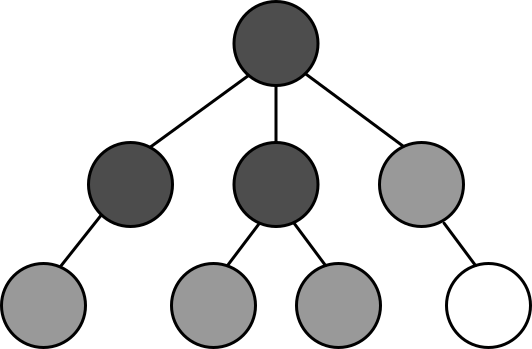
\includegraphics[scale=0.4]{Images/bfs_search.png}
    \caption{Example of vertex colouring for BFS}
    \label{fig:bfs-example}
\end{figure}

\begin{lstlisting}
BFS(G = (V, E), s):
    # we first initialise the graph with appropriate values
    for v in V:
        colour[v] = white
        d[v] = inf # distance from s/depth of node in BFS tree
        p[v] = null # parent, pi is another commonly used symbol
    
    # initialising s
    colour[s] = grey
    d[s] = 0
    initialise empty queue Q # Q will store the grey vertices, handled in FIFO order
    ENQUEUE(Q, s)
    
    while Q is not empty:
        u = DEQUEUE(Q, s)
        for each edge (u, v) in E:
            if colour[v] == white:
                colour[v] = grey
                d[v] = d[u] + 1
                p[v] = u
                ENQUEUE(Q, v)
        colour[u] = black
\end{lstlisting}

Let us consider the complexity of this algorithm. First we see that each node is enqueued at most once (namely if it is connected to $s$ or reachable from $s$). So the while loop iterates at most $|V|$ times. Moreover the while and for loop combined iterate over all the edges in $G$. Therefore the run time of this algorithm is $O(|V| + |E|)$ (if $|E| < |V|$ then we might still need to iterate over all the vertices so we again have the case that the runtime is bounded by the larger of the two).\\

We claim that the BFS satisfies a very neat property: namely the $d[u]$ of each vertex after the algorithm is shortest distance from $s$ to the vertex $u$. By definition this is the smallest number of edges on any path from $s$ to $u$ (this definition will alter slightly when we consider weighted graphs). 

Let $\delta(s, v)$ denote the shortest distance between $s$ and $v$. First we claim that $\delta(s, v) \leq \delta(u, v) + 1$ for all $(u, v) \in E$. This is obvious if $v$ is not reachable from $s$ (this means that if $(u, v) \in E$ then $u$ is not reachable from $s$ so the right hand side is $\infty$). Suppose $v$ is reachable from $s$ then. Suppose $p$ is a path from $s$ to $v$. If we remove the last edge from $p$, we get a path from $s$ to some $u$. By definition, the length of this path must be greater than or equal to $\delta(s, u)$ (remember that $\delta(s, u)$ is the length of the shortest path so all other paths must be bigger or equal in length). Then the length of $p$ is at least $\delta(s, u) + 1$. Once again we use the definition of $\delta$ to conclude that $\delta(s, v) \leq \delta(s, u) + 1$.

Next we claim that $d[v] \geq \delta(s, v)$ for all $v \in V$ at any point during BFS. Clearly this holds at the beginning (line 14) as $d[s] = 0 = \delta(s, s)$ and $d[v] = \infty$ for all other $v$. We inductively assume the claim holds for some sequence of \ttt{ENQUEUE} and \ttt{DEQUEUE} operations and we will show it holds immediate after one of these operations as well. Suppose we enqueue a vertex $v$. Then we must have discovered it from a vertex $u$ which was queued before. Therefore $d[u] \geq \delta(s, u)$. Additionally by line 19 of the algorithm, we know that $d[v] = d[u] + 1$, allowing us conclude that $d[v] \geq \delta(s, u) + 1$ which we know to be greater than or equal to $\delta(s, v)$ by the previous lemma. Since we never change $d[v]$ again, the claim holds.

The next lemma is that if $Q = [v_1, \dots, v_r]$ then $d[v_i] \leq d[v_{i + 1}]$ and moreover that $d[v_r] \leq d[v_1] + 1$. This mean that the distances in the queue at any time are non-decreasing and can differ by at most 1. We will induct similarly to before. Clearly this holds in the base case when $Q = [s]$ (there is only one element!). So suppose the statement holds when $Q = [v_1, \dots, v_r]$ and we will show it holds whenever we \ttt{ENQUEUE} or \ttt{DEQUEUE} from this point. Dequeuing is the easier one to consider. Since we are assuming $Q$ to be non-decreasing to be begin with, removing $v_1$ doesn't change this and $v_2$ is made the new first element (or $Q$ is empty now which is also fine). Since $v_1 \leq v_2$ and $v_r \leq v_1 + 1$, we must have that $v_r \leq v_2 + 1$ preserving the second property. Now suppose we enqueue a vertex $v$, making it now $v_{r+1}$. By looking at the code, we see that this occurs after dequeuing its parent $u$. Then $d[v] = d[u] + 1$. By assumption $d[u] \leq d[v_1]$ therefore $d[v] = d[v_{r + 1}] \leq d[v_1] + 1$. By assumption we know that $d[v_r] \leq d[v_1] + 1$ so the non-decreasing property is maintained as well.

\begin{theorem}
After we run BFS(G, s), $d[v] = \delta(s, v)$ for every $v \in V$.
\end{theorem}
\begin{proof}
We prove this using contradiction. Let $v$ be a vertex where $d[v] > \delta(s, v)$ for the minimum such $\delta(s, v)$ (we already know that $d[v]$ cannot be less than $\delta(s, v)$ by the first claim shown above). This means that for all $u$ where $\delta(s, u) < \delta(s, v)$ then $d[u] = \delta(s, u)$. Let $u$ be $v$'s preceding vertex in the minimal path from $s$ to $v$. Then we know that $d[u] = \delta(s, u)$ (indeed it is not hard to see that $\delta(s, u) = \delta(s, v) - 1$). Thus our assumption is equivalent to $d[v] > d[u] + 1$.

Now suppose we have dequeued vertex $u$ and are exploring the edge $(u, v)$. There are three possible colourings that $v$ could have. If $v$ is white then $d[v]$ is set to $d[u] + 1$ (and never reset to anything else), leading to a contradiction. If $v$ is black, then it appeared in the queue before $u$ so $d[v] \leq d[u]$ (remember we have non-decreasing distances in $Q$). This leads us to another contradiction. The final possibility is that $v$ is grey. This means $v$ is currently in $Q$ (this is where all the grey vertices are stored). Then before $u$ was dequeued, $u$ and $v$ were simultaneously in $Q$. We know then that $d[v] \leq d[u] + 1$ (distances in the queue can differ by at most 1) giving us our final contradiction.
\end{proof}

\subsection{Depth First Search}
As we said depth first search will be the counterpart to breadth first search. In this case, we will search as deep as possible before backtracking to explore the edges of an already discovered vertex. We will also be colouring the vertices as we walk through the graph and the colours and what they correspond to will be the same: white for undiscovered vertices, grey for discovered vertices that have not been fully explored and black for vertices that have been fully explored. In this case, however, our definition of fully explored is subtly different. We will say a vertex has been fully explored if we have explored all of its its children and their children and their children and so on. Additionally instead of storing a distance in the nodes we will store two timestamps (i.e. two integers) for the discovery time, when a vertex is first discovered, and the finish time, when a vertex has been fully explored.

DFS is an algorithm that is begging to be written recursively. Hence we will heed its wishes and do just that. Additionally, DFS is commonly used to find the connected components so our main algorithm won't take in a source vertex will instead call a helper function \ttt{DFS-VISIT(G, u)} repeatedly for each $u$ in $V$. 

\begin{lstlisting}
DFS(G = (V, E)):
    # initialisation
    for each v in V:
        colour[v] = white
        f[v] = d[v] = inf
        p[v] = null
    time = 0 # global
    
    for each v in V:
        if colour[v] == white:
            DFS-VISIT(G, v)

DFS-VISIT(G = (V, E), u):
    colour[u] = grey
    time = time + 1
    d[u] = time
    
    for each (u, v) in E:
        if colour[v] == white:
            p[v] = u
            DFS-VISIT(G, v)
    colour[u] = black
    time = time + 1
    f[u] = time
\end{lstlisting}
\begin{remark}
The above algorithm is for a directed graph. For undirected graphs, we just need to make a slight tweak to ensure that we don't travel over the same edge twice.
\end{remark}

After we have run DFS we will be left with a whole bunch of disconnected trees, which is called the DFS-forest. Specifically, we will have trees from the parent-child relationships we are tracking, each of which corresponds to an edge in the original graph. These edges are called, understandably enough, tree edges. However consider the remaining edges in the graph. We may, for example, have a \textit{back edge} $(u, v) $ where $v$ is an ancestor of the vertex $u$ (hence we are going `back up' the tree with this edge). These are found during the execution of line 19 above, when the colour of an edge's endpoint (in this case $v$) is grey. We may of course have cases where rather than being an ancestor $v$ is a descendant of $u$. In this case we get a \textit{forward edge}. Finally, we may have that $v$ is neither an ancestor nor a descendant. Thus the edge $(u, v)$ is an edge between different branches of the same tree or an edge between different trees in the forest. Such edges are called cross-edges. Both forward edges and cross-edges are found when $v$ is black.

% TODO: Add back edges and forward edges and cross edges

Let us consider the complexity of DFS. Note that \ttt{DFS-VISIT} is only called on white vertices which are immediately painted grey. So \ttt{DFS-VISIT} is called exactly once on each vertex (note this is different from BFS since in a disconnected graph, we may not reach every node with BFS. With DFS, however, this is not the case). Each \ttt{DFS-VISIT} also walks through the adjacency list of a single vertex. Hence over all the vertices we will have traversed through all the edges. As we have argued before, the complexity of this algorithm must then be the larger of $\left| V \right|$ and $\left| E \right|$, so in particular we can conclude that the runtime for DFS is $O(\left| V \right| + \left| E \right|)$.

We have one final property with DFS known as the parenthesis theorem. 
\begin{theorem}[Parenthesis theorem]
Suppose we run DFS on a graph $G$. Then for any vertices $u, v \in G$, exactly one of the following holds:
\begin{itemize}
    \item $\left[d[u], f[u]\right] \cap \left[d[v], f[v]\right] = \emptyset$: the two intervals are disjoint
    \item $\left[d[u], f[u]\right] \subset \left[d[v], f[v]\right]$: the interval $\left[d[u], f[u]\right]$ is contained in $\left[d[v], f[v]\right]$
    \item $\left[d[v], f[v]\right] \subset \left[d[u], f[u]\right]$: the interval $\left[d[v], f[v]\right]$ is contained in $\left[d[u], f[u]\right]$
\end{itemize}
\end{theorem}

\subsection{Using DFS}
Topological sort is a way of ordering vertices, specifically in directed, acyclic graph. In particular, it is a linear ordering of vertices so that if $(u, v)$ is an edge in $G$, then $u$ comes before $v$ in the ordering (this shows why we need the graphs to be directed and acyclic). Using DFS, an algorithm to find a topological sorting of the vertices is quite easy to find. In particular, we perform DFS and as each vertex finishes we add it to the beginning of the list. This works because a vertex is added only after all its edges have been explored fully. Thus by adding it to the beginning we know that all of its neighbours will only appear later in the list.

DFS can also be used to determine whether or not a directed graph $G$ is strongly connected, where by strongly connected we mean that for every pair of vertices $u, v$ there is a path from $u$ to $v$ and from $v$ to $u$ (this is very similar to the idea of connectedness for undirected graphs, although, as you might imagine, a bit more work needs to be done for strong connectedness since we need paths to exist in both directions). In order to find an algorithm for this, we employ the classic trick when handed a difficult problem: reduce it to a simpler one. Note that being strongly connected is equivalent to saying that there exists a node $s$ such that there is a node from $s$ to every vertex and a path from every vertex to $s$ (we can then construct a path from $u$ to $v$ by combining the paths from $u$ to $s$ and from $s$ to $v$). Of course if a graph is strongly connected then every $s$ is going to satisfy this property, so we can choose a vertex $s$ at random and simply check whether or not it satisfies this property.  

The question then remains how can we check this. Well, at least one of the directions is easy to do with DFS. Namely, we perform \ttt{DFS-VISIT(s)}. If $f[s] = 2|V|$, then we know there is a path from $s$ to every other vertex. This is because the timer increments once each time we encounter a new vertex and once each time the vertex has been fully explored. Thus if $f[s] = 2|V|$, then all the vertices in $G$ were encountered (thus if $f[s] < 2 \left|V\right|$, we know that $G$ is not strongly connected). Thus if $f[s] = 2\left|V\right|$, we know that every vertex is reachable from $s$. But how can we determine whether the reversal of this question is true, whether $s$ is reachable from every vertex? In fact, phrasing this as the reversal is exactly the way to think of this: we simply reverse all of the edges in $G$ and run the same algorithm on this new graph. In this way, if a vertex is reachable from $s$ in the new graph, $s$ is reachable from the vertex in the original one. As a side note, the reversal of all the edges is particularly simple with adjacency matrices: we simply take their transpose!

\subsection{Minimum Spanning Trees}
Given a graph $G$, a spanning tree is a tree (i.e. an undirected, acyclic, connected graph), formed from a subset of the graphs edges that contains all the vertices in $G$. Quite often there is more than one spanning tree. In the case of unweighted graphs, all spanning trees are (generally) equally optimal. If the edges have weights though, this is no longer the case. In particular, there will be a \textit{minimum spanning tree}.

Given a weighted graph $G$, we can talk about its own weight (sometimes denoted $w(G)$) which is simply the sum of the weights of the edges in the graph. Then a minimum spanning tree for $G$ is a spanning tree whose weight is smaller than or equal to the weight of any other spanning tree. The minimum spanning tree (MST) need not be unique either (the trivial example is any unweighted graph, which can be viewed as a weighted graph where all the edges have the same weight. In this call, all spanning trees will have the same weight).

A very common problem is to find a minimum spanning tree of a weighted graph. The general approach for our algorithms to achieve this will be to start with just the vertices and continually add edges from the the graph to make a tree or forest as we go until we have our MST. Thus in general, the algorithm can be described like so
\begin{lstlisting}[language=]
GREEDY-MST(G = (V, E), w):
    T = {} # invariant: T is a subset of some subset of G
    while T is not a spanning tree: # i.e. while |T| < |V| - 1:
        find e "safe for T"
        T = T + e # or T = T union {e}
\end{lstlisting}
where \ttt{w} is the weight map, i.e. a map from the set of edges $E$ to the real numbers. Also note how in this case, we are thinking of the tree as simply a set of edges.

The question, of course, is what does it mean for an edge to be safe. To be honest, the precise definition is that $e$ is safe for $T$ if $T$ being a subset of a minimum spanning tree implies that $T \cup \{e\}$ is also a subset of a minimum spanning tree. This is a bit of circular definition, so we need another way of determining when an edge is safe. For this we have the following theorem.
\begin{theorem}
Suppose $G$ is a connected, undirected, weighted graph, $T$ is a subset of some MST of $G$ and $e$ is an edge whose endpoints lie in different connected components of $T$. If $e$ is an edge of minimal weight connecting the connected components, then $e$ is safe for $T$.
\end{theorem}
Intuitively, this theorem is clear. Given two connected components in $T$, we know that the MST must contain an edge connecting them and if we pick an edge which doesn't have the minimal weight, then it would not be a \textit{minimum} spanning tree. We use this theorem for both the algorithms below, albeit in different ways.

\subsubsection{Prim's Algorithm}
Prim's algorithm works by choosing an initial root vertex and continually adding edges of minimal weight to $T$ to form a growing tree. That is, at each step we find an edge that has one vertex in $T$ and one outside $T$ and moreover over all such edges, we pick the edge that has minimal weight. The algorithm written precisely is like so:
\begin{lstlisting}
MST-PRIM(G = (V, E), w, r):
    # r = initial choice of root
    # initialisation
    for each v in V:
        priority[v] = inf # we will use a priority queue to determine the edge to add
        p[v] = None # p[u] = parent of node u
    priority[r] = 0
    Q = V # Q = our priority queue
    
    # main bit
    while Q is not empty:
        u = ExtractMin(Q)
        T = T + {(p[u], u)} # unless when u = r (in which case p[u] doesn't make sense)
        for each v in adj[u]:
            if v in Q and w(u, v) < priority[v]:
            # w(u, v) < priority[v] means that we have found a `shorter'/more optimal path to v
            decreasePriority(Q, v, w(u, v))
            p[v] = u
\end{lstlisting}
Importantly, note the use of the method \ttt{decreasePriority} in line 17. This is of course not a part of the Priority Queue ADT (see \autoref{sec:heaps}), so we must augment our data structure. It is not immediate how we should change the heap data structure to allow for changing priorities. The main problem is of course finding the particular element, after finding the element, we just need to do some bubble ups. Luckily we don't need to do any searching! We can simply assume that the \ttt{v} in line 17 has a pointer to the corresponding element in the heap, which means that \ttt{decreasePriority} is $O(\log \left| V \right|)$ in the worst case (since the number of elements in the heap is $\left| V \right|$). Additionally, the combination of the \ttt{while} loop in line 11 and the \ttt{for} loop in line 14 means that the \ttt{if} block is run at most $\left| E \right|$ times (the combination of the loops means we iterate over $|E|$ twice since edge will be found once from either end point. But each edge can only be added at most once and after an edge has been added the \ttt{v in Q} part of the \ttt{if} statement will evaluate to false once we reach it a second time. This implies that the overall runtime of this algorithm is $O(\left|E\right| \log \left|V\right|)$.

\subsubsection{Kruskal's Algorithm}
Kruskal takes a slightly different approach. Instead of starting with a tree and maintaining it throughout, Kruskal starts with a forest and continually adds edges until we form a tree. The claim is that the tree at the end will be a minimum spanning tree of the initial graph. What edges should we add to ensure that this claim holds? As you might imagine it is the edge of minimal weight that we add. Once again, to be precise, at each step we pick the minimal edge among all the remaining edges that do not form a cycle. We form a cycle exactly when both end points of the edge are in the same connected component in $T$. Thus, we can describe the algorithm like so
\begin{lstlisting}
MST-KRUSKAL(G = (V, E), w):
    # as before w = weight function/assignment
    T = {}
    sort edges so that w(e_1) <= w(e_2) < ... <= w(e_m)
    for i in range(1, m + 1):
        let (u_i, v_i) = e_i
        if u_i and v_i are in different connected components of T:
            T = T + {e_i}
\end{lstlisting}

We know that the sorting in line 4 can be done in $O(\left|E\right| \log \left|E\right|)$ time. The big question, of course, is how can we determine efficiently whether or not two vertices are in the same connected component. For this, we turn to a new data structure!

\section{Disjoint Set ADT}
The data for the disjoint set ADT is a collection of non-intersecting sets where each set is identified by a unique element of the set called the representative. Thus we can determine whether two elements are in the same set by comparing their representative (or more precisely by comparing the representatives of the sets that the two elements belong to).

Given the context from Kruskal's algorithm, it seems natural to have the following operations for this ADT:
\begin{itemize}
    \item \ttt{Make-Set(x):} Given an element $x$ that is not already in one of the disjoin sets, create a new set containing only $x$ and designate $x$ as the representative of this set.
    \item \ttt{Find-Set(x):} Given an element $x$, return the representative of the set that $x$ belongs to (or NIL if $x$ belongs to none of the sets).
    \item \ttt{Union(x, y):} Given elements $x$ and $y$ that belongs to the sets $S_x$ and $S_y$, make a new set $S_x \cup S_y$, designate a representative and remove $S_x$ and $S_y$ from the ADT (the last part is necessary to maintain disjointedness of the sets)
\end{itemize}
\begin{remark}
It is also useful (and important) to note what is \textit{not} possible with this data structure. For example, there is no way of finding what all the disjoint sets are or of finding what all the elements in a given disjoint set are.
\end{remark}
With this, we can make the pseudocode a bit less informal
\begin{lstlisting}
MST-KRUSKAL(G = (V, E), w):
    T = {}
    sort edges so that w(e_1) <= w(e_2) < ... <= w(e_m)
    for v in V:
        Make-Set(v)
    for i in range(1, m + 1):
        let (u_i, v_i) = e_i
        # if u_i and v_i are in different connected components of T:
        if Find-Set(u_i) != Find-Set(v_i):
            Union(u_i, v_i)
            T = T + {e_i}
\end{lstlisting}

It is important to realise how the disjoint set ADT is typically implemented: in particular each element maintains a pointer to the DJS data structure.

We will look at various ways of implementing DJS analysing each one by the worst case sequence complexity.

\subsection{Implementation I: Circular linked list}

% TODO: Include diagram for DJS implementation 1

We might initially start with each disjoint set being a linked list with the final element having a pointer back to the first element (thereby forming the circular structure). We designate one of the elements in the linked list as the representative (marking it in some way) so that \ttt{Find-Set} simply requires iterating through the list until we find the representative. \ttt{Union} is a bit more finnicky (we are trying to combine two loops into one loop. The procedure is as you would expect but to execute it takes some work.).

Suppose the set $S_x$ contains $x_1, \dots, x_n$ and the set $S_y$ contains $y_1, \dots, y_m$ (where $S_x$ and $S_y$ are both stored as circular linked lists) with $x_1$ and $y_1$ as the respective representatives. Then running \ttt{Union}($x_2, y_5$), for example, we link $x_2$ to $y_5$ (i.e. the next element of $x_2$ now points to $y_5$). Then we iterate through $S_y$ to find the element preceding $y_5$, namely $y_4$, and link $y_4$ to $x_3$ (and remove the pointer from $y_4$ to $y_5$ of course). This forms one continuous loop. The only problem is that this set now has two representative but this can be dealt with easily by demarking (unmarking?) the representative in $S_y$ as we were iterating over it.

\begin{remark}\label{rem:impl1-convention}
Quite often, instead of linking $x_3$ to $y_5$ we might instead link $x_n$ to $y_1$ and $y_n$ to $x_1$. Ultimately of course the result is the same (we still get one continuous loop of $S_x \cup S_y$) and takes about the same time. With this implementation of \ttt{Union}, the result of unioning an element of $S_x$ with an element of $S_y$ will always produce the same result (for example the resulting linked list with \ttt{Union}($x_2$, $y_5$) and as the linked list with \ttt{Union}($x_4, y_1$)). 
\end{remark}

Let us analyse this implementation using worst case sequence complexity. Note that in a sequence of $m$ operations we can get a set to contain at most $m$ elements and \ttt{Find-Set} will need to iterate over most $m - 1$ items on such a set (if we call it on the element immediately after the representative for example). Thus immediately we find that the worst case sequence complexity is $O(m^2)$ (this would correspond to calling \ttt{Find-Set} on the set of $m$ elements $m$ times. Clearly this is a very large upper bound since simply constructing a set of $m$ elements would require more than $m$ operations). 

We claim that the worst-case sequence complexity is in fact $\Theta(m^2)$. For this we need to give a family of sequences which actually achieves the $m^2$ runtime. The idea is to actually achieve the sequence that was suggested in the upper bound argument above. Namely, we will use the first portion of the sequence to construct a large set and then use the latter portion of the sequence to call expensive \ttt{Find-Set} operations. To be precise, the first $n$ operations in the sequence are \ttt{Make-Set}'s, where $n = \frac{m}{4}$. The following $\frac{m}{4} - 1$ operations are unions so that we can combine these $n$ elements into one big set (this portion of the sequence might look something like \ttt{Union}($x_1, x_2$), \ttt{Union}($x_1, x_3$), \dots, \ttt{Union}($x_1, x_n$)). The remainder of the sequence is \ttt{Find-Set}($x_2$) (remember the convention described in \autoref{rem:impl1-convention}). In this case, the \ttt{Find-Set}'s will each require $\Theta(n) = \Theta(\frac{m}{4})$ runtime. Since there are $\frac{m}{2} + 1$ such \ttt{Find-Set}'s, these operations alone will require $\Theta(m^2)$ runtime giving the desired tight bound.

\subsection{Implementation II: Backpointers}

% TODO: Include diagram for DJS implementation 2

The problem with the above implementation is that some \ttt{Find-Set}'s take too long. We might consider fixing this by including a pointer to the representative in every node. In this manner, \ttt{Find-Set} would run in constant time! The problem, as you might imagine, is union. In particular, we would need to change the pointers for all the elements in the second set. 

We can similarly argue that the worst case sequence complexity for this implementation is $\Theta(m^2)$. As before, we argue that there at most $m$ elements in any disjoint set, thus union requires changing at most $m$ pointer. Thus if the sequence was all \ttt{Union}'s and it \textit{did} have to change $m$ pointers each time, we would get a quadratic runtime. Clearly the runtime for a sequence of length $m$ must smaller than this, allowing us to conclude that that the worst case sequence complexity is $O(m^2)$. We can also construct a sequence to conclude that the worst case sequence complexity is $\Theta(m^2)$. As before, we will try achieve the worst case scenario painted previously. We will take $n = \frac{m}{2}$ and have the first $n$ operations be \ttt{Make-Set}'s. The following $\frac{m}{2} - 1$ operations are \ttt{Union}'s where the second element is always the larger one (as an example, this sequence might look something like \ttt{Union}($x_2, x_1$), \ttt{Union}($x_3, x_1$), ..., \ttt{Union}($x_n, x_1$)). The number of pointers changed over all the unions is 
$$ \sum_{i = 1}^{\frac{m}{2} - 1} i = \Theta(m^2) $$

Side note: the sequence defined above is of length $m - 1$. You can have the last operation be anything to get the sequence to be of length $m$. It doesn't really matter since the unions defined above take $\Theta(m^2)$ on their own.

\subsection{Implementation III: Union by Weight}
There is an obvious improvement to the above implementation. Instead of always changing the pointers in the second set, we should instead change the pointers in the smaller of the two sets. To this end, we add an attribute to each disjoint set called the weight, which is simply the number of items in the set.

Now for the worst case sequence complexity analysis. In this case we will only be able to find an upper bound rather than a tight bound. Let $x$ be any element in one of the disjoint sets. We want to find the number of times the pointer from $x$ to its representative will change. Note that the pointer only changes when $x$ is in the smaller of the two sets. In such cases the size of the set that $x$ is in at least doubles. Thus $x$ is going to be in the smaller set at most $\log n$ times where $n$ is total number of elements in all of the disjoin sets. Since each element's pointer is changed at most $\log n$ times and there are $n$ elements, at most $n \log n$ pointers are changed. Since \ttt{Make-Set} and \ttt{Find-Set} are both constant time, we find that the worst case runtime of a sequence of $m$ operations with this implementation is $O(m + n \log n)$ where $n$ is the number of \ttt{Make-Set} operations in the sequence (if there are lots of \ttt{Make-Set} and \ttt{Find-Set} operations instead of \ttt{Union} operations, then $m$ is going to be greater than $n \log n$, thereby dominating the runtime. Otherwise we have $O(n \log n)$ runtime). 

\subsection{Implementation IV: Inverted Tree}
Having played around with this a fair amount by now, we might realise that it seems unnecessary to add lists and combine loops to form larger loops, when all we really need is some way of getting to the representative from any given node. Thus for instance when taking union of two sets, why not have the representative of the second one point to the representative of the first one. Furthermore, having forward pointers is largely unnecessary when again all we need is a way to get to the representative. Instead we could reverse the forward pointers so there is a path from every node to the representative.

To summarise, we have the following: we have a tree structure with the representative as the root. However, the tree is inverted since the rather than have parents point to children, we have children point to parents. We will also have the root point to itself.

% TODO: Add diagram for implementation 4

With this implementation, \ttt{Make-Set} is of course constant. \ttt{Find-Set} in the worst case is going to be $\Theta(h)$ where $h$ is the height of the tree. Finally \ttt{Union} is simply the time for \ttt{Find-Set} plus some constant amount of changing pointers. 

As usual, we will do our worst case sequence complexity analysis. As before it is easy that worst case runtime must be $O(m^2)$ (\ttt{Find-Set} takes at most $\Theta(m)$ time, for example if we call it on a leaf of the tree and the tree has no branches). The sequence we provide is the one that more or less actualises this worst case scenario. Namely we have $n = \frac{m}{4}$ \ttt{Make-Set} operations and $\frac{m}{4} - 1$ \ttt{Union}'s in such a way so that the resulting tree is simply a chain (this can be done by making the first argument to \ttt{Union} a singleton set every time). Then we call \ttt{Find-Set} on the very last item each time for the remaining operations giving us $\Theta(m^2)$ runtime in the worst case.

\subsection{Implementation V: Inverted Tree with Union by Weight}
We can of course make the same improvement we made last time: namely each tree stores its weight (i.e. the number of nodes in it) and when performing a union we ensure that the larger tree is one whose root/representative is maintained (note that larger trees will have more leaves and \ttt{Find-Set} is most expensive on leaves. So in order to minimise the number of leaves after the union we keep the larger tree as the root). 

We can run a similar analysis to before. Let $x$ be any arbitrary element in one of the disjoint sets. The distance between $x$ and its representative only increases if it is unioned with a larger set. By previous argument, we know that this can happen at most $\log n$ times (where $n$ is total number of elements). Note that each step distance between $x$ and and its representative only increases by 1. Since at the beginning $x$ is its own representative, we know that the height of any tree in the data structure can be at most $\log n$ after $m$ operations, $n$ of which were \ttt{Make-Sets}. This means that each \ttt{Find-Set} takes at most $O(\log n)$ thus the worst case time complexity of a sequence of $m$ operations is $O(m \log n)$. 

\subsection{Implementation VI: Path Compression}
Ideally, what we would like is for the tree to always be of height 1 with each node pointing directly to the representative. But as you might imagine that is going to be quite hard to maintain. For example upon performing a union we would have to go through all the children of the root and change their pointers to the new one (and we don't even have a way of finding all the children! Remember all the pointers are reversed so we only have pointers from children to their parents). A better idea is to update these pointers when we find them. In particular, suppose we call \ttt{Find-Set} on an element and see that it doesn't point to the root. Then we follow the path to the root and modify all the nodes along the path so that they all point directly to the root. This is known as \textit{path compression}. Admittedly this might double the runtime for \ttt{Find-Set} (if an element is at depth $d$, then it takes $d$ steps to get to the root and since there are $d$ elements along the way (including itself), we have $d$ pointers to change as well) but it means that all future operations are much cheaper. A messy proof tells us that the sequence complexity with path compression is $O(m \log m)$. 

% TODO: Add diagram for path compression

\subsection{Implementation VII: Union by Rank}
With path compression, it is not the weight of the tree that is important but its height. Thus we will track the height instead of the weight. But then we realise that keeping track of the height exactly is actually quite difficult. Performing a path compression may or may not have decreased the height; the only way to know would be know the depths of all the leaves (which would involve keeping track of the leaves as well, at least roughly). Luckily we don't need to known the height exactly, simply knowing an upper bound for it will do. This quantity is known as the rank. It can also be defined like so: the rank of a leaf is always 0 and the rank of an internal node is 1 more than the maximum rank of its children.

We need to check how rank interacts with the ADT operations. If we do \ttt{Make-Set}($x$), then it is clear that we should set the rank of the node to be 0 (remember that the rank of a leaf is 0). The rank remains unchanged after running \ttt{Find-Set} (if anything the height will have decreased, but the upper bound will still hold so it need not be changed). When performing a \ttt{Union} we ensure that it is the representative of higher rank that becomes the root in which case the rank need not changed (the upper bound is still maintained). If, however, the rank of the two representatives is the same, then taking the union \textit{will} could increase the maximum height, by 1, and therefore we also need to increase the rank by 1. In this scenario, we could pick either representative to be the root, but by convention we will always choose it to be the first one. 

An even messier proof than before shows that the worst case sequence complexity for this implemenetation is $O(m \log^* n)$ where $\log^*$ is the \href{https://en.wikipedia.org/wiki/Iterated_logarithm}{iterated logarithm}. $\log^* n$ is the number of times that the logarithm function must be applied to $n$ in order to get a result that is below 1. To be formal, you can define it as
\begin{align*}
    \log^*(n) = 
    \begin{cases}
    0 \ & n \leq 1\\
    1 + \log^*(\log n) & n > 1
    \end{cases}
\end{align*}
Note that $\log^*$ is a very, very slow growing function. The function is 0 on $(-\infty, 1]$, 1 on $(1, 2]$, 2 on $(2, 4]$, 3 on $(4, 16]$, 4 on $(16, 65536]$, 5 on $(65536, 2^{65536}]$ and so on. Thus the function is essentially constant meaning that the amortised complexity with this algorithm is very close to being constant.

\section{Lower Bounds}
Lower bounds are some of the most delightful things in computer science. In this case you analyse, not the complexity of a particular algorithm, but the complexity of a problem, in order to make statements about the minimum amount of effort required to solve a problem. In other words, you are finding what is the smallest runtime that \textit{any} algorithm solving the problem could have. 

Consider the example of sorting. We know we can sort in $O(n \log n)$ (via randomised quicksort for example). This gives an upper bound for the runtime of the best algorithm for sorting. If we knew the lower bound we could conclude that we had already found the best algorithm (up to asymptotic behaviour). But this is clearly a difficult problem: we would need to argue that \textit{every} algorithm solving the problem must run a certain amount of time. In practice, to make our lives easier we often classes or families of algorithms (i.e. algorithms that tackle the problem in similar ways). 

To continue the example with sorting, consider the class of algorithms that use pairwise comparison (i.e. the sorting is done by comparing pairs of elements in some manner). We can use comparison trees to represent such algorithms. 

\subsection{Comparison Trees}
In order to get used to arguing with comparison trees, let us consider the slightly different problem of searching through a sorted (1-based index) list and returning the index of the item if present. Suppose we are searching for an element in $x$ in a list $A$ where $A$ is of length 3. In the first step, we compare $x$ with $A[2]$ to determine whether $x$ should be on the first half of the list or the second half. Then we compare $x$ with $A[1]$ or $A[3]$ depending on the previous result (but not both). Now we know that $x$ is either at a specific index or not in the list at all. We can determine which of these it is with one final comparison. We can summarise all this in a comparison tree, see \autoref{fig:search-compar-tree}.

\begin{figure}[h]
    \centering
    
\includegraphics[scale=0.55]{Images/search_compar_tree.png}
    \caption{Comparison tree for binary search (return 0 if $x$ is not in the list)}
    \label{fig:search-compar-tree}
\end{figure}

Suppose a problem has $q$ possible outputs. This puts a lower bound on the height of the comparison tree since each output will correspond to at least one leaf. In particular, recall that a binary tree of height $h$ can have at most $2^h$ leaves. Conversely, if a binary tree is to have $q$ leaves then it must at least be of height $\lceil \log q \rceil$. The worst case runtime is proportional to the height of the tree and the expected runtime is proportional to the average depth of the leaves.
\begin{remark}
This means that searching in a sorted list with $q$ items is going to take at least $\Omega(\lceil \log (q + 1) \rceil) = \Omega(\log q)$ time. But binary search already has this runtime so we confirm that binary search is the fastest way of searching in a sorted list!
\end{remark}

\subsection{Sorting}
We now apply a similar analysis to the problem of sorting. First we make the problem precise: we seek an algorithm that will take as input a list of length $n$ and output a permutation of $[1, \dots, n]$ indicating the position (or rank as in \autoref{sec:aug-data-struc}) of each element. Thus for example, the output for $[2, 6, 3]$ would be $[1, 3, 2]$. The comparison tree for $n = 3$ might look like \autoref{fig:sorting-compar-tree}.

\begin{figure}[h]
    \centering
    
\includegraphics[scale=0.5]{Images/sorting_compar_tree.png}
    \caption{Comparison tree for sorting with $n = 3$}
    \label{fig:sorting-compar-tree}
\end{figure}

There are $n!$ possible outputs (the number of permutations of $[1, \dots, n]$) thus the height of comparison tree must be at $\log n!$. We claim that $\log n! = \Theta(n \log n)$ since
\begin{align*}
    \log n! &= \log n + \log(n - 1) + \dots + \log 2 + \log 1 \leq n \log n\\
    \log n! &= \log n + \log(n - 1) + \dots + \log 2 + \log 1 \geq \log n + \log(n - 1) + \dots + \log \frac{n}{2} \geq \frac{n}{2} \log \frac{n}{2}
\end{align*}
Thus any sorting algorithm that uses pairwise comparisons must take at least $\Theta(n \log n)$ time.

One does occasionally hear whispers of sorting being done in much faster time. How is this possible? The answer is cheating (kind of). We have found the lower bound for a very particular problem, if we change the problem slightly, for example by adding certain restrictions, we can get different lower bounds. A somewhat silly example is if we knew the elements of the list to be sorted were $n$ distinct elements from $[1, \dots, n]$. In this case, the algorithm could be made constant time by simply returning the input list. 


\end{document}
